%\documentclass[11pt, twoside]{article}
\documentclass[11pt]{article}

\usepackage{amsmath} 
\usepackage{times}
\usepackage{amsmath,amsthm,amssymb}
\usepackage{enumerate}
\usepackage{fancyhdr}
\usepackage{moreverb}
\usepackage{graphicx}
\usepackage{verbatim}
\usepackage{amssymb}
\usepackage{url}
\usepackage{multirow} 
\usepackage[boxed, section]{algorithm}
\usepackage{algorithmic}
\usepackage{cite}
\usepackage{multirow} 
\usepackage{rotating}
\usepackage{geometry}
\usepackage{fix-cm}
\usepackage{natbib}
 \usepackage{setspace}
\usepackage{caption}
\usepackage{subcaption}
\usepackage{color}
\usepackage[T1]{fontenc}
\usepackage[utf8]{inputenc}
\usepackage{authblk}

\newcommand{\myN}{\hbox{N\hspace*{-.9em}I\hspace*{.4em}}}
\newcommand{\myZ}{\hbox{Z}^+}
\newcommand{\myR}{\hbox{R}}
\renewcommand{\P}{\mathbb{P}}
\newcommand{\E}{\mathbb{E}}
\newtheorem{defi}{Definition}
\newtheorem{theorem}{Theorem}[section]
\newtheorem{lemma}[theorem]{Observation}
\newtheorem{observation}[theorem]{Observation}
\newtheorem{proposition}[theorem]{Proposition}
\newtheorem{claim}[theorem]{Claim}
\DeclareMathOperator*{\argmax}{arg\,max}

\theoremstyle{definition}
\newtheorem{example}[theorem]{Example}
\theoremstyle{definition}
\newtheorem{definition}[theorem]{Definition}

\renewcommand{\abstractname}{}
\def\pb{\overline{p}}
\def\pt{\tilde{p}}
\def\one{{\bf 1}}
\def\F{{\cal F}}
\def\G{{\cal G}}
\def\P{{\mathbb P}}
\def\E{{\mathbb E}}
\def\Var{{\rm Var}\,}
\def\Cov{{\rm Cov}\,}
\def\ee{\varepsilon}
\def\|{\, | \,}
\def\probit{p_{\rm probit}}
\def\plog{p_{\rm log}}

%\doublespacing

%%%%%% Begin document with header and title %%%%%%%%%

%\title{Combining Probability Forecasts and Understanding Probability Extremizing through Information Diversity}
\title{Modeling Probability Forecasts via Information Diversity}
\author[1]{Ville A. Satop\"a\"a\thanks{Corresponding author. tel.: +1 215 760 7263; fax: +1 215 898 1280; email: satopaa@wharton.upenn.edu}}
%\author[2]{Robin Pemantle\thanks{pemantle@math.upenn.edu}}
%\thanks{Research supported by NSF award \# DMS-1209117}
%\author[3]{Lyle H. Ungar\thanks{ungar@cis.upenn.edu}}
\author[2]{Robin Pemantle\thanks{Research supported in part by NSF grant
   \# DMS-1209117}}
\author[3]{Lyle H. Ungar}
\affil[1]{Department of Statistics,
The Wharton School of the University of Pennsylvania\\
400 Jon M. Huntsman Hall\\
3730 Walnut Street\\
Philadelphia, PA 19104-6340}
\affil[2]{Department of Mathematics\\
University of Pennsylvania\\
David Rittenhouse Laboratories\\ 
209 S. 33rd Street\\
Philadelphia, PA 19104-6395 }
\affil[3]{Department of Computer and Information Science\\
University of Pennsylvania\\
504 Levine, 200 S. 33rd Street\\
Philadelphia, PA 19104-6309}
\date{\vspace{-10ex}}


\begin{document}
\maketitle
\pagestyle{myheadings}
\markboth{Understanding Probability Extremizing}{Satop\"a\"a et al.}
\begin{abstract}
\noindent
\textbf{Summary.} Randomness in scientific estimation is generally 
assumed to arise from unmeasured or uncontrolled factors. However, 
when combining subjective probability estimates, heterogeneity
stemming from people's cognitive or information diversity is often
more important than measurement noise.  This paper presents a novel
framework that models the heterogeneity arising from forecasters that use 
partially overlapping information sources, and applies that model to 
the task of aggregating the probabilities given by a group of forecasters 
who forecast whether an event will occur or not. Our model describes 
the distribution of information across forecasters in terms of easily
interpretable parameters and shows how the optimal amount
of \textit{extremizing} of the average probability forecast (shifting
it closer to its nearest extreme) varies as a function of the forecasters'
information overlap.  Our model thus gives a more principled
understanding of the historically {\it ad hoc} practice of extremizing
average forecasts.\\
\\
\textit{Keywords:} Expert Beliefs; Information Aggregation; Model Averaging; Probability Forecasting; Stochastic Process; Wisdom of Crowds
\end{abstract}


\section{Introduction and Overview}

\subsection{The Forecast Aggregation Problem}

Event forecasting is the science of giving probability forecasts
for future events.  The classical examples can be found in meteorology
\citep{sanders1963subjective}, where the scientists are often interested in accurate probability predictions of different weather phenomena such as rain in the next few days.
But the practice has now spread to many other fields as well. This includes
medical diagnosis and prognosis \citep{wilson1998prediction,pepe2003statistical, o2006uncertain}, estimation of credit default \citep{kramer2006evaluating}, and
predicting political and socio-economic events \citep{tetlock2005expert} such as who will win the next Congolese election, or whether war will break out in Egypt this year. Accurate probability forecasts on such events are important for the decision-maker who wants to decide, for instance, what to pack for tomorrow's family outing or whether to advice against all travel to Egypt. 

The decision-maker, however, often has access to several different forecasts on the same event. For instance, one forecast might draw its information from television news in the United States while the other is based on local news in Egypt. In such cases, bringing together the
strengths of different forecasters by combining their forecasts has been shown to improve predictive
performance under various contexts~\citep{clemen1989combining, armstrong2001combining}. Unfortunately, the choice of the combination rule can have a large impact on the predictive quality of the final aggregate forecast. 
%Analyzing and developing improved rules is the main motivation of 
This motivates \textit{forecast aggregation} that is the problem of combining two or more forecasts into a single forecast with optimal properties. 

There are two general approaches to forecast aggregation: empirical
and theoretical.  The empirical approach is akin to machine
learning. Given a training set with several forecasts on events with known outcomes, the decision-maker experiments with several aggregation techniques and chooses the technique (and potentially any parameter values) that yield the best performance on the training set. 
 The theoretical approach, on the other hand, first produces a probability
model and then computes the optimal aggregation procedure under the 
assumptions of the model.  This may involve estimating model parameters from the forecasts. 

Both approaches are important.  Procedures based on theory that
do not perform well in practice are ultimately of limited use.
On the other hand, an empirical approach without theoretical
underpinnings lack both credibility (why should we believe it?)
and guidance (in which direction can we look for improvement?).
As we will discuss below, the history of forecast aggregation
to date is largely empirical\footnote{Not only the approaches in
Section~\ref{ss:empirical} but also the approaches described in
Section~\ref{ss:measurement}, to which we have provided theoretical 
underpinnings, have been pursued in a manner that is largely empirical.}.  
The goal of this paper is to
produce a plausible theoretical framework for forecast aggregation.
This framework allows us to interpret existing aggregation 
procedures and illuminate aspects that can be improved.
Secondly, at a general level, we use this framework to shed light on 
the practice of {\em probability extremizing} (shifting an average aggregate closer to its nearest extreme). This is an empirical technique that has been widely used to improve the predictive performance of many simple aggregators such as the average probability. Thirdly, we apply
this framework to a specific model, where the optimal 
aggregator may be computed.

\subsection{Bias, Noise and Forecast Assessment}
\label{BiasNoise}
Represent the event to be forecasted with an indicator function that equals one or zero depending whether the event happens or not, respectively. Each probability forecast is then an estimator of this indicator function.  As is
the case with any estimator, their deviation from the truth
can be broken into two pieces: bias and noise.  In the forecasting literature, a forecaster
 is said to be {\em calibrated}
if, in the long run, events associated with a forecast $p \in [0,1]$ have an empirical frequency of occurrence of $p$ (see, e.g., \citealt{degroot1983comparison}). For instance, consider all events that the forecaster believes to occur with a 60\% probability. If the forecaster is well-calibrated, 60\% of these events will actually end up occurring. The same, of course, has to be true across all probabilities -- not just 60\%. 
In the lingo of estimation, this is equivalent to being conditionally 
unbiased.  

Non-expert populations are typically not calibrated. There are, however, many subpopulations of experts that are highly calibrated. For instance, meteorologists performing probabilistic weather forecasting have been found to be calibrated (\citealt{murphy1977reliability}); experienced tournament bridge players were highly calibrated in predicting whether a contract would be made (\citealt{keren1987facing}); and bookmakers generally give calibrated forecasts on sports events (\citealt{dowie1976efficiency, yates1985conditional}). If the decision-maker is left with poorly calibrated forecasts, they can, in principle, be corrected by translating the forecast $p$ into the forecast $\pt$
where $\pt$ is the (historical) proportion of times the 
event occurs when $p$ is forecast.  One can then assume without
loss of generality that the forecaster is calibrated, replacing
$p$ if necessary by the historically corrected $\pt$. This assumption is, of course, valid only in principle: 
it relies on a relatively lengthy history and an assumption
of stationarity of the properties of the forecasts.
% For other calibration techniques, see, for instance, \citealt{foster1998asymptotic, Brier}. 
 Nevertheless,
on the theoretical level, it is important to separate the problems 
of bias and noise because they are solved by different mechanisms.
In this paper we consider the aggregation problem for calibrated forecasts, thus isolating the task to one of noise reduction. 

Before delving into the problem of forecast aggregation, it is useful to briefly discuss the problem of assessing and improving a single
forecast stream.  The most common methodology is to use a loss
function.  Letting $\one_A$ denote the indicator function of the
event $A$ being forecast, the loss function is a penalty 
$L(p , \one_A)$ where $p$ is the forecasted probability.
A loss function is said to be {\em revealing} or {\em proper}
if the Bayesian optimal strategy is to tell the truth.  In other words, 
if the subjective probability estimate is $p$, then $t = p$ should
minimize the expected loss $p L(t,1) + (1-p) L(t,0)$.  This expected loss is a one dimensional
assessment of an estimator. Many
choices, however, are possible, and an estimator that outperforms 
another under one loss function will not necessarily do so
under a different loss function.  For example, minimizing the quadratic loss function
$(p - \one_A)^2$, also known as the {\em Brier score}, gives the estimator with the least variance. On the other hand, minimizing the entropy loss $\log (1 / |p - \one_{A^c}|)$ reveals the estimator that best avoids forecasting an incorrect event with near 
certainty; see~\citet[Section~2]{HwPe1997} for a discussion of
proper loss functions.

The point of this brief review is two-fold.  First, when a group of
sophisticated forecasters operates under a revealing loss function,
the assumption of calibrated forecasts is, to some degree, 
self-fulfilling.  Forecasters can improve their long run 
performance by calibrating their forecasts. Forecasters with 
competitive motivation, sophistication and historical data
will probably do so. In fact, calibration has been noticed to improve via training and active feedback (see \citealt{o2006uncertain} for an excellent overview of calibrating subjective probability forecasts). Secondly, the assessment of the aggregated forecast
is not uni-dimensional any more than is the assessment of an
individual forecast.  In order to compare different aggregation 
procedures, a scoring rule must be chosen.  In practice, the
Brier score is the most common choice, perhaps because of its simplicity
or because of the paramount status of variance in the statistical
literature.  In this paper we will concentrate on minimizing the
variance of aggregators, though much of the discussion will hold under
general proper loss functions.

\subsection{The Partial Information Framework}
\label{PIFintro}
The construction of any probability model for forecast aggregation must begin with a 
probability space $(\Omega, \F , \P)$ and a measurable event
$A \in \F$ to be forecasted.  In any Bayesian setup, with a proper 
loss function, it is more or less tautological that a forecaster
reports $p = \E (\one_A \| \G)$ where $\G \subseteq \F$ is the
\textit{information set} used by the forecaster.  The \textit{partial information framework} extends this idea to 
$N$ forecasters. In particular, it posits the existence
of sub-$\sigma$-fields $\F_i \subseteq \F$ such that Forecaster~$i$
forecasts $p_i = \E (\one_A \| \F_i)$. 

The information sets contain only information actually used by the forecasters. This means that if Forecaster $i$ uses a simple rule, the $\sigma$-field $\F_i$ may 
not be the full $\sigma$-field of information available to 
Forecaster~$i$ but rather a smaller $\sigma$-field corresponding
to the information actually used by the rule.  For example, 
when forecasting the chances of the president being re-elected,
a forecaster obeying the dictum ``it's the economy, stupid!''
might be assigned a $\sigma$-field containing only economic indicators. 
This is reminiscent of a forecasting algorithm that uses a similarly restricted subset
of the information fed to it. Therefore any heterogeneity in the forecasts stems purely  from \textit{information diversity}.  Anything further must come from
assumptions on the structure of the collection $\{ \F_i : i = 1, \dots, N\}$.
%%%In Section~?? we explore in detail a particular such structure.

To illustrate, suppose that the forecasters face a sequence of
 events $\{ A_1, A_2 , \ldots \}$. The general  framework only assumes that Forecaster~$i$ uses some 
$\sigma$-field $\F_{ij}$ to make a probability forecast for event $A_j$.  Further aspects of the problem are
reflected by the structure of the collection $\{ \F_{ij} \}$.
For example, if the events are sequenced in time, then the information sets
$\{ \F_{ij} : j = 1 , 2, 3, \ldots \}$ are likely to form an increasing 
sequence.  If the forecasts are public, it may make sense to 
assume that $\F_{ij}$ contains all forecasts up to time $j-1$.
%If, in addition, the forecasts of each individual event $A_j$ are sequenced rather 
%than synchronous, the set $\F_{ij}$ may contain information about
%some forecasts at time $j$ as well. 
This is, of course, only one illustration. The framework itself is quite flexible yet intuitive. In fact, it is not difficult to imagine a wide variety of other forecasting setups and how their specifications translate to different inter-dependencies among the information sets.




The partial information framework distinguishes two benchmarks for efficiency in
aggregation.  The first is the {\em oracular} aggregator $p' := \E (\one_A \| \F')$, where $\F'$ is the $\sigma$-field
generated by the union of the $\sigma$-fields $\{ \F_i : i = 1, \dots, N\}$.  Obviously, it is not possible do better when forecasting the
probability of the event $A$ than to use all the information available 
to the forecasters; note that if a forecaster chooses to throw away 
some of the available information then, for purposes of aggregation,
the information may as well not exist.  The oracular aggregator
is a reasonable model for an upper bound on estimation efficiency;
information not in $\F'$ represents randomness inherent in the outcome. 

In practice, however, the aggregator cannot necessarily do as well as the oracular aggregator.  This is because information comes to the aggregator only via the forecasts. Therefore, in practice, the 
aggregator cannot improve upon the estimate $p'' := \E (\one_A \| \F'')$,
where $\F''$ is the $\sigma$-field generated by the forecasts
$\{ p_1 , \ldots , p_N \}$. This estimate is the second benchmark aggregator. It is named the {\em revealed} aggregator 
because it uses exactly the information revealed by the forecasters
through their forecasts.  Furthermore, it minimizes the expectation of any proper scoring rule (\citealt{Ranjan08}), and, unlike the oracular aggregator, can be applied in practice. For this reason, in each specific partial information model, the relevant estimator 
is the revealed aggregator. 




%The {\em general partial information model} 
%is precisely the model described in the foregoing paragaphs.  
%Specific partial information models involve assumptions on
%the structure of $\{ \F_i \}$.  In each case, the relevant estimator 
%is the revealed aggregator. 

\subsection{Organization of the Paper}

The next section reviews some prior work on aggregation and 
indicates the relation to the partial information framework.
Section~\ref{sec:model} discusses some illuminating examples 
and motivates our subsequent choices of specific partial information 
models.  Section~\ref{extremizing} compares the oracular
aggregator $p'$ with the probit opinion pool $\probit$, thereby
explaining the empirical practice of {\em probability extremizing}.
Section~\ref{aggregation} derives the revealed aggregator for a
particular partial information model and evaluates it on real-world forecasting data.  The final section concludes with a discussion of future research.



\section{Some Prior Work on Aggregation}
\label{sec:prior}

Prior work on aggregation has focused on non-quantitative
frameworks that explain heterogeneity of subjective forecasts.  
The following subsections discuss two of these approaches. 

\subsection{The Interpreted Signal Framework}
\label{ss:inerpreted}

\citet{hong2009interpreted} adopt the {\em interpreted 
signal framework} in which the forecaster's opinion is based on a personal
interpretation of (a subset of) the factors or cues that influence
the future event to be predicted.  Differences among forecaster
predictions are ascribed to differing interpretation procedures.
For example, if two forecasters follow the same political campaign
speech, one may focus on the content of the speech while the other 
may concentrate largely on audience interaction.  Even though the
two candidates both receive the same information, they interpret
it differently, arriving at different forecasts for the probability
that this candidate wins the election.  

Therefore forecast heterogeneity is assumed to
stem from cognitive diversity.  This is a realistic framework that
has been analyzed and extended to many other settings.  For example,
~\citet{parunak2013characterizing} demonstrate that optimal aggregation of
forecasts in this model is not constrained to the convex 
hull of the forecasts;~\citet{broomell2009experts}
analyze inter-forecaster correlation
under the assumption that the cues can be mapped to the individual
forecasts via different linear regression functions.

The interpreted signal framework, when formalized, more or less implies 
the partial information framework.  Unfortunately, previous work on
interpreted forecasts has produced only abstract concepts and 
has not been taken to the level of a precise formal model with 
quantitative predictions.  Given this lack of a quantitative model, in practice it is often easier and more common to explain subjective
forecasts with the {\em measurement error framework}. This framework is described in the next subsection.

\subsection{The Measurement Error Framework}
\label{ss:measurement}
The measurement error framework assumes a ``true'' probability $\theta$ (interpreted
as the probability forecast made by an ideal forecaster) for the future 
event.  The forecasters are able to measure this probability but with
some mean-zero idiosyncratic error.  This is formalized by modeling each forecast
as a draw from a common probability distribution that is typically 
centered at the true probability.  
%
Therefore the underlying probability model is just the classical statistical
model for measurement with i.i.d. mean zero error.  Consequently, the average probability, $\pb = \frac{1}{N}\sum_{i=1}^N p_i$,
is an aggregator that is unbiased for $\theta$ and has the least variance.

Different versions of this model alter the quantity that is supposedly 
measured without bias. For example, if instead of the true probability $\theta$,
the true log odds $\log\left\{\theta/(1-\theta)\right\}$ have been measured without bias, 
the average log odds will be an unbiased estimator. Transforming this average back into
an estimate for $\theta$ yields the {\em logarithmic opinion pool}
$$\plog := \frac{\exp \left [ \frac{1}{N} \sum_{i=1}^N
   \log \left\{ p_i / (1-p_i) \right\} \right ]}
{1 + \exp \left [ \frac{1}{N} \sum_{i=1}^N
   \log \left\{p_i / (1-p_i)\right\} \right ]} $$
This aggregator has been analyzed and utilized by many investigators
(see, e.g., \citealt{dawid1995coherent, Genest, bacharach1975group}). Alternatively, target quantity can be the true probit $\Phi^{-1}(\theta)$, where $\Phi$ represents the cumulative distribution function (CDF) of a standard Gaussian distribution. This gives rise to the {\em probit opinion pool} 
$$\probit := \Phi \left\{ \frac{1}{N} \sum_{i=1}^N \Phi^{-1}
   (p_i) \right \} $$

% In this case, the underlying probability model assumes that the forecasters are able
%to observe  the true probit score with i.i.d. mean zero error.
%%%The probit transformation is favored in economics, while other disciplines
%%%more commonly  use the log-odds transformation~(\citet{bryan2013regression}).
%%%The choice is usually made based on computational convenience
%%%versus ease of interpretation: the log-odds are considered more
%%%interpretable, while probit can be more convienient if reported
%%%forecasts are already standardized.
These aggregators illustrate the main advantage of this model: simplicity.  The formula
for a new aggregator is obtained in a straightforward manner by 
transforming, averaging, and transforming back.  The underlying probability
model is also simple and very familiar.  There are, however, a number
of disadvantages.  First, these \textit{averaging aggregators} target the mean of (potentially transformed) probability forecasts. The correct target, however, is the random quantity $\one_A$ that lies on the boundary of the sample space. Important properties, such as calibration, cannot be expected from an aggregator that is based on a model that does incorporate a link between the observations and the correct quantity of interest. This makes the measurement error framework inherently inappropriate for probability aggregation. 


Second, the introduction of a nonlinear 
transformation biases the estimator.  Therefore neither $\plog$ 
nor $\probit$ produces a calibrated forecast. Exactly how
problematic this is depends on whether the bias is small enough
to be swamped by the noise or other adjustments.  The direction of
the bias can sometimes be determined. For instance, \citet{Ranjan08} prove that any convex combination of calibrated forecasts will be under-confident, that is, too close to $1/2$. This result applies to the averaging aggregators because they are by nature different convex combinations of the forecasts. 

A third and more serious disadvantage is the implausibility of the underlying 
model. Introducing a ``true'' probability is vulnerable to many philosophical debates, and even if one eventually manages to convince one's self of the existence of such a parameter, it is difficult to believe that the forecasters
are actually seeing the hidden parameter $\theta$ (or $\log\{\theta/(1-\theta)\}$ 
or $\Phi^{-1}(\theta)$) with independent noise. Therefore, whereas the
interpreted signal framework proposes a micro-level explanation,
the measurement error model does not; at best it forces us to 
imagine that the forecasters are all in principle trying
to apply the same procedures to the same data but are making
numerous small mistakes in their observations or their application 
of the procedures.  

A fourth disadvantage is that the averaging aggregators are often not very good.  For one thing,
any transformed average is constrained to the convex hull of the
individual forecasts.  As previously mentioned, this contradicts the 
interpreted signal model \citep{parunak2013characterizing}.  Empirically, one sees for many data 
sets that an aggregator restricted to the convex hull will be far 
from optimal. See Example \ref{FirstExample} for a simple illustration of this. 

\subsection{Empirical Approaches}
\label{ss:empirical}

If one is not concerned with theoretical justification, an obvious
approach is to perturb one of these estimators and observe 
whether the adjusted estimator performs better on some data set
of interest.  It is known both theoretically and empirically
that the measurement error framework produces under-confident 
aggregators.  A popular adjustment, therefore, is to {\em extremize},
that is, to apply a post-transformation that shifts the 
aggregated forecast closer to the nearer extreme (either zero or one).
For instance,~\citet{Ranjan08} propose transforming
the (weighted) average $\pb$ with the CDF of a beta distribution.  If both the shape and scale of this 
beta distribution are equal and constrained to be at least~1.0,
the aggregator extremizes and has some attractive theoretical
properties~\citep{Wallsten2001}.  ~\citet{satopaa}
use a logistic regression model to derive an aggregator that extremizes
the average log-odds.  ~\citet{baron2014two} give two intuitive
justifications for extremizing and discuss an extremizing technique
that has previously been used by a number of investigators~\citep{Erev1994,
shlomi2010subjective}; one could perhaps trace this all the way back
to~\citet{karmarkar1978subjectively}.  
In an empirical study,~\citet{mellers2014psychological} show that 
extremizing can improve the quality of aggregate forecasting of 
international events.  
%%%\citet{turner2013forecast} and \citet{Ariely00theeffects} 
%%%also mention the benefits of extremizing.

This places the current state-of-the-art aggregators in an unwieldy
position.  They first compute an average based on a model that
is likely to be at odds with the actual process of probability
forecasting, then aim to correct this misalignment via {\em ad hoc} 
extremizing techniques.  
%
Not only does this leave something to be desired from an explanatory 
point of view, such an approach is also subject to the problems of 
machine learning, such as overfitting.  For example, many currently
used aggregators learn the amount of extremizing by optimizing a scoring
rule over a separate training set (see~\citealt{Gneiting04strictlyproper} 
for a discussion on scoring rules).
Given that such a training set requires repeated realizations of
a single event, it is not clear how these aggregators can be applied
for a one-time event. Overall, while {\em ad hoc} extremization works to some degree, such
techniques provide little insight beyond the amount of extremizing
itself.  They do not point the way to continued improvement.

The present paper aims to remedy this situation.
The framework of partial information produces theoretically
based estimators which explain extremization.  We produce a 
simple instance of partial information in which the amount of 
extremization can be quantified with a single number
that follows a Cauchy distribution.  Given that this distribution
depends on a structure of information among the forecasters, it establishes
a link between the information structure and the amount of
extremizing one must apply to an averaging aggregator.  This leads
to three main results.  First, the modal amount of extremizing is 
increasing in the level of information diversity and the total amount 
of information among forecasters.  Second, no matter how information is 
distributed among forecasters, extremizing the probit opinion pool
is more likely to be beneficial than harmful (except in the degenerate
situation where all forecasts are the same). Third, the structure of the information overlap among the forecasters establishes a spectrum of aggregators, ranging from average- (most information is public) to voting-like (most information is private) techniques. 


\section{The Gaussian Partial Information Model}
\label{sec:model}

\subsection{Motivating Examples}

Partial information models are sensitive to the structure of 
information overlap that is assumed to hold among the individual 
forecasters.  Model sensitivity is good when it reflects
sensitivity to important inherent features of the problem,
but bad when it adds noise that is not reflected in the
actual best response to the data.  It therefore behooves
us to begin with some simple examples to show that the best
aggregate forecast is not well defined without assumptions
on the information structure among the forecasters.

\begin{example}
\label{FirstExample}
Suppose two forecasters both forecast a probability of $2/3$ for
some event.  If they are seeing the same evidence, then the best
aggregate forecast probability is $2/3$.  If they are seeing
different evidence, then clearly the combined evidence should give
an aggregate forecast somewhat greater than $2/3$.  To make the
situation more concrete, suppose that the event to be forecasted is that
a coin, picked from a basket containing a fair coin and a two-headed
coin, is in fact two-headed.  Each forecaster observes the result
of a single flip of the coin that was picked.  If they see HEADS,
then the correct Bayesian probability estimate is $2/3$.  If both
forecasters see the result of the same coin flip, then the best
aggregate probability estimate is again $2/3$.  If they observe
different (presumably independent) coin flips, then the best
aggregate probability estimate is $4/5$.  
\end{example}

The point of this example is that, based on just these observations, 
there is no way to distinguish the two situations.  If we are able
to observe these two forecasters for a longer time, we might be
able to ascertain whether they tend to have the same information.
Had the two forecasts in the above example disagreed, we would be
sure they were not seeing the same coin flip.  However, in the given
situation, there was no way to know, and neither $2/3$ nor $4/5$ 
can be said to be a better choice than the other for an aggregate
forecast.  We conclude that it is necessary to add an assumption
as to the information overlap structure, and that this must be
informed by the particular instance of the problem. The next example shows that even when we assume two forecasters to observe
independent events, further details as to the structure of information
can still greatly affect the optimal aggregate forecast.  

\begin{example}
Let 
$\Omega = \{ A,B,C,D \} \times \{ 0,1 \}$ be a probability space 
with eight points.  Let $\mu$ be the measure assigning 
probabilities $\mu (A,1) = a/4, \mu (A,0) = (1-a)/4$, 
$\mu (B,1) = b/4, \mu (B,0) = (1-b)/4$, and so forth.
Let $\F_1$ be the $\sigma$-field containing $S_1$ and its complement, 
where $S_1 = \{ (A,0),(A,1),(B,0),(B,1) \}$ is the
event that the first coordinate was $A$ or $B$.  Let $\F_2$
be defined similarly, but for the event $S_2$ that the first coordinate
is $A$ or $C$.  These two $\sigma$-fields are independent.
Let $G$ be the event that the second coordinate is~1.
Forecaster~1 will forecast the following probabilities for $G$:
if the observed first coordinate is $A$ or $B$, then
the forecast will be $(a+b)/2$, otherwise it will be $(c+d)/2$.
Forecaster~2 will forecast the following probabilities for $G$:
if the observed first coordinate is $A$ or $C$, then
the forecast will be $(a+c)/2$, otherwise it will be $(b+d)/2$.
If $\ee$ is added to $a$ and $d$ and subtracted from $b$ and $c$,
none of the forecasts change, nor does it change that each of
the four possible pairs of forecasts has probability $1/4$.
Therefore, all observables are invariant under this perturbation.
If Forecasters $1$ and $2$ report $(a+b)/2$ and $(a+c)/2$, respectively, then the aggregator knows that
the first coordinate is $A$.  Consequently, the optimal aggregate forecast is $a$.  This is most definitely affected by the perturbation.  
\end{example}

The point of this example is that the aggregation problem is 
affected by the fine structure of shared information.  It is, however,
unlikely that the structure can ever be known with the precision
postulated in this toy model.  Therefore we will need to make
reasonable assumptions, yielding plausible and generic information
structures.

\subsection{Gaussian Partial Information Model}
\label{ss:Gaussian}

\begin{quote}
{\bf The Model.} Let $S = [0,1]$ denote 
the unit interval and let $\{ X_B \}$ be a centered Gaussian process 
on some abstract space $(\Omega , \F , \P)$, indexed by the 
Borel subsets of $B \subseteq S$, with covariances $\Cov (X_B , X_{B'}) 
= |B \cap B'|$.  In other words, the unit interval is endowed
with Gaussian white noise and $X_B$ is the total of the white
noise in the Borel subset $B$.  Let $A$ denote the event that
the sum of all the noise is positive: $A := \{ X_S > 0 \}$.
For each $1 \leq i \leq N$, let $B_i$ be some Borel subset of $S$,
and let $\F_i := \sigma (X_{B_i})$.  Let $p_i := \E (\one_A \| \F_i)$.
\end{quote}

To motivate and interpret this model, recall the 
interpreted signal model of~\citet{broomell2009experts}, in which 
different forecasters use different linear functions of the data.  
In other words, there are observable quantities $Z_1 , \ldots , Z_r$, 
and Forecaster~$i$ forms an opinion based on $L_i (Z_1 , \ldots , Z_r)$, 
where each $L_i$ is a linear function.  Proposing a linear model
for subjective interpretation seems quite natural and is in fact
the only such postulate we know to have been suggested for 
interpreted signals.
If the observables (or any linear combination of them)
are independent and have small tails, then as $r \to \infty$, the
joint distribution of linear combinations $L_1 , \ldots , L_N$
will be asymptotically Gaussian.  Given that the number of cues affecting the forecaster's decision on real-world problems is likely to be large, it makes sense to model
the forecasters' observations as jointly Gaussian.  The following
observations provide interpretation and clarify which aspects of the
Gaussian model are essential and which have little or no impact.

\begin{enumerate}[(i)]
\item {\bf Interpretations.} It is not necessary to assume anything 
about the source of the information.  For instance, the information 
could stem from photographs, survey research, records, books, 
interviews, or personal recollections.  All these details have 
been abstracted away.

\item {\bf Information Sets.} The set $B_i$ holds the information used by Forecaster $i$, and the covariance  $\Cov (X_{B_i} , X_{B_j})$ represents the information overlap between the Forecasters $i$ and $j$. 
%\item In the interpreted signal framework, the set $B_i$ represents 
%the linear regressor used by Forecaster~$i$, and the covariance 
%structure represents degrees of similarities between regressors 
%of different forecasters.  
Consequently, the complement of $B_i$ holds 
information not used by Forecaster~$i$.  No assumption is necessary
as to whether this information was unknown to Forecaster~$i$ instead of
known but not used in the forecast.


\item {\bf Pool of Information.} The role of the unit interval is for convenient 
specification of the sets $B_i$. The pool of information potentially
available to the forecasters is the white noise on $S$. The choice of unit interval is not relevant, and any other set could have been used. There is
no sense of time or ranking of the information within the pool. Instead,
the pool is a collection of information, where each piece of information
has an {\em a priori} equal chance to contribute to the final outcome.
Quantitatively, the information is parametrized by the length measure on $S$.


\item {\bf Invariant Transformations.}  From the empirical point of view, the exact identities of the individual 
sets $B_i$ are irrelevant.  All that matters are the covariances $\Cov \left(X_{B_i} , X_{B_j}\right)  
= |B_i \cap B_j|$.  The explicit sets $B_i$ are for use in the theoretical
analysis.

\item {\bf Scale Invariance.} The model is invariant under rescaling, replacing $S$
by $[0,\lambda]$ and $B_i$ by $\lambda B_i$.  Therefore, the
actual scale of the model (e.g., the fact that the covariances of 
the variables $X_B$ are bounded by $1$) is not relevant. 


\item {\bf Specific versus General Model.} A specific model 
requires a choice of an event $A$ and Borel sets $\{ B_i : i = 1, \dots, N\}$.  
This might be done in several ways:
a) by choosing them in advance, according to some criterion;
b) estimating the parameters $\P(A)$, $|B_i|$ and $|B_i \cap B_j|$
from the data; c) using a Bayesian model with a prior distribution on the unknown parameters.  
This paper focuses mostly on (a) and (b) but discusses (c) shortly in 
Section~\ref{discussion}.  Section \ref{extremizing} provides one result, namely 
Proposition~\ref{positiveProbThm}, on the general model, 
holding for any (nonrandom) choices of the sets $\{ B_i : i = 1, \dots, N\}$.
\label{item:specific}






\item {\bf Choice of Target Event.}  There is one substantive assumption 
in this model, namely the choice of the half-space $\{ X_S > 0 \}$ 
for the target event $A$.  Changing the target event results in a 
non-isomorphic model. The current choice of the half-space implies a prior probability $\P(A) = 1/2$, which seems as uninformative as possible and therefore provides a natural starting point. Specifying a prior distribution for $A$ cannot be avoided as long as the model depends on a probability space. As was mentioned in Section \ref{PIFintro}, this includes essentially any probability model for forecast aggregation.  

\item {\bf Centering.} One could choose a non-central halfspace 
$\{ X_S > t \}$ for $A$, where $t \neq 0$.  This would make the 
the prior probability of $A$ different from $1/2$.  This paper focuses on the 
centered model for simplicity but also for the following reason.  
The Gaussian assumption is most often true in practice when the 
observations are centered.  Therefore, for example, if the electorate 
is broken into a dozen demographic segments, the portion of voters 
in each segment that vote for a given candidate does not follow a 
Gaussian distribution, but the difference between this portion and 
the historically expected or predicted portion may.  A centered 
partial information model is then quite realistic when forecasting 
the event of a positive deviation.  The political futures website, Intrade, 
during its operation, was in fact well stocked with centered events, 
such as the event that the number of representatives elected from 
a given party would exceed a threshold (the threshold being adjusted 
to bring this probability near $1/2$).  Sports betting websites operate 
almost exclusively in this mode.
\label{item:centered}
\end{enumerate}

\subsection{Preliminary Observations}
\label{prelim}
This section describes the details of the Gaussian partial information model. It is helpful to begin the introduction by considering only 
two forecasters.  That is, consider, Forecasters $1$ and $2$ who see respective 
$\delta_1$ and $\delta_2$ portions of the Gaussian process. 
These portions form their information sets.  Let $\rho$ denote
the size of the overlap of the two information sets.
Therefore, if $I_1, I_2 \subseteq S$ denote the information 
sets observed by Forecasters $1$ and $2$, respectively, then
\begin{align*}
|I_1| &= \delta_1\\
|I_2| &= \delta_2\\
|I_1 \cap I_2| &= \rho
\end{align*}
\begin{figure}[htbp]
%   \hspace{-2em}
   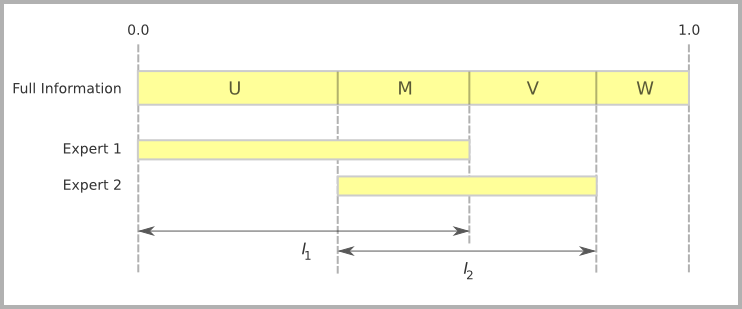
\includegraphics[width = \textwidth]{N=2} % requires the graphicx package
   \caption{Illustration of the partial information model with $2$ forecasters.}
   \label{diagram2}
\end{figure}
Figure \ref{diagram2} illustrates this setup.  In this diagram the 
Gaussian process has been partitioned into four parts based on the 
forecasters' information sets:
\begin{align*}
 U &= X_{I_1 / I_2}
& M &= X_{I_1 \cap I_2}\\
 V &= X_{I_2 / I_1}
& W &= X_{(I_1 \cup I_2)^c}
\end{align*}
Then,
\begin{align*}
X_{I_1} &= U + M\\
X_{I_2} &= M + V\\
X_S &= U+M+V+W,
\end{align*}
where $U, V, M, W$ are independent Gaussians with respective variances 
$\delta_1-\rho$, $\delta_2-\rho$, $\rho$, $1+\rho-\delta_1 - \delta_2$. 
The random variable $X_{I_i}$ can be interpreted as the information 
known by Forecaster $i$.  The joint distribution of $X_{S}$, $X_{I_1}$, 
and $X_{I_2}$ is a multivariate Gaussian distribution.  That is,
\begin{align}
\left(\begin{matrix} X_S \\ X_{I_1}\\ X_{I_2} \end{matrix}\right) 
 &\sim \mathcal{N}\left(
 \boldsymbol{0},  \left(\begin{matrix} 
1 & \delta_1 & \delta_2\\
\delta_1 & \delta_1 &\rho\\
\delta_2 & \rho & \delta_2
 \end{matrix}\right)\right) \label{twoforecasters}
\end{align}
Given that $X_S$ has mean zero, the prior probability for the event 
is $\P(X_S > 0) = \P(A) = 1/2$.  As was mentioned above in Remark (\ref{item:centered}), 
this can be easily adjusted to any probability $\tilde{p}$ by 
letting $A = \{ X_S > \Phi^{-1}(1-\tilde{p}) \}$.  In this paper, however,
we limit our attention to the centered model with prior probability $1/2$.

\begin{figure}[htbp]
   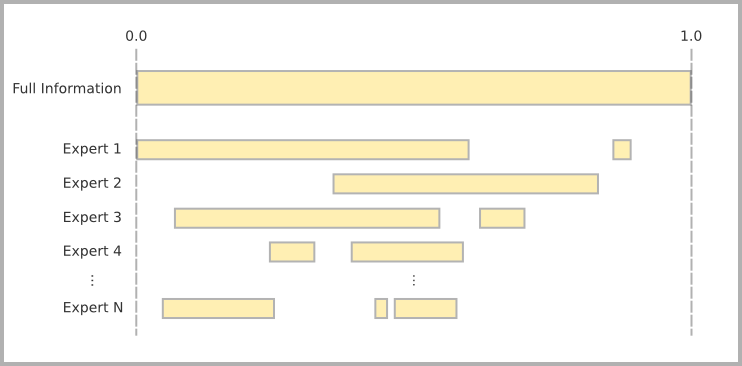
\includegraphics[width = \textwidth]{N=N} % requires the graphicx package
   \caption{Illustration of the partial information model with $N$ forecasters.}
   \label{diagramN}
\end{figure}

Consider now $N$ forecasters. Let $|I_i| = \delta_i$ be the amount of 
information known by Forecaster $i$ for $i = 1, \dots, N$, and 
$|I_i \cap I_j| = \rho_{ij} = \rho_{ji}$ be the information overlap 
between Forecasters $i$ and $j$ with $i \neq j$. 
Expression~(\ref{twoforecasters}) generalizes to the vector 
$\left(X_{S}, X_{I_1}, X_{I_2}, \dots, X_{I_N}\right)$ as follows.
\begin{align}
\left(\begin{matrix} X_S \\ X_{I_1}\\ \vdots \\ X_{I_N} \end{matrix}\right) &\sim \mathcal{N}\left( \left(\begin{matrix} 
\mu_1 \\ \boldsymbol{\mu}_2
 \end{matrix}\right) =
 \boldsymbol{0}, \left(\begin{matrix} 
\Sigma_{11} & \Sigma_{12}\\
\Sigma_{21} & \Sigma_{22}\\
 \end{matrix}\right) 
 =
 \left(\begin{array}{c | c c cc }
1 & \delta_1 & \delta_2 & \dots & \delta_N  \\ \hline
\delta_1 & \delta_1 &\rho_{1,2} & \dots & \rho_{1,N}   \\ 
\delta_2 & \rho_{2,1} & \delta_2 & \dots & \rho_{2,N}  \\ 
\vdots & \vdots & \vdots & \ddots & \vdots  \\ 
\delta_N & \rho_{N,1} & \rho_{N,2} & \dots & \delta_N\\ 
 \end{array}\right)\right)  \label{Nforecasters}
\end{align}
This case is illustrated in Figure \ref{diagramN}.  It is important 
to notice that $I_i$ does not have to be a contiguous segment of 
the unit interval.  Instead, each forecaster can know any Borel measurable 
subset of the full information.  Given that the information structure 
is described by the sub-matrix $\Sigma_{22}$, learning about the 
information among the $N$ forecasters is equivalent to estimating 
a covariance matrix under several restrictions.  First, each element 
of $\Sigma_{22}$ must be in the unit interval, and no off-diagonal 
element can be larger than the corresponding diagonal element in 
the same row. Second, $\Sigma_{22}$ must be symmetric, non-singular, 
and coherent. The matrix $\Sigma_{22}$ is coherent if and only if 
its information structure can be described by a diagram such as 
the one given in Figure \ref{diagramN}. 


The next step is to link this model with the probability forecasts. 
If $P_{I_i} = X_{I_i}/\sqrt{1-\delta_i}$ represents the probit 
forecast made by Forecaster $i$, the corresponding probability forecast is given by
\begin{align}
p_i &= \P\left(A | \mathcal{F}_{I_i}\right) = \Phi\left( P_{I_i}\right) 
\label{Indiv}
\end{align}
These forecasts are calibrated. 
%Let $A_1, A_2, \dots$ be a infinite sequence of events, each defined 
%similarly to $A$.  If the $i$th forecaster's probability forecast for 
%$A_j$ is given by~(\ref{Indiv}), then the forecaster's forecasts are
%calibrated.  Given that several experiments have shown that forecasters 
%are often poorly calibrated (see, e.g.,~\citealt{cooke1991forecasters, 
%shlyakhter1994quantifying}), assuming calibrated forecasts can be 
%unrealistic.  If the forecasters make repeated forecasts for a sequence 
%of events (e.g., whether it rains or not over a series of days), 
%it may be possible to calibrate their forecasts (see, 
%e.g.,~\citealt{foster1998asymptotic, Brier}).  If calibration is not 
%possible, systematic bias can be introduced in the model by 
%changing the total information by an amount unknown to the forecasters. 
%Another alternative is to include an additive error term 
%in~(\ref{Indiv}) such that the forecasters are on average calibrated. 
%These extensions, however, are beyond the scope of this paper. 
The marginal distribution of $p_i$ is
\begin{align*}
m(p_i | \delta_i) &= \sqrt{\frac{1-\delta_i}{\delta_i}} \exp 
   \left\{ \Phi^{-1}(p_i)^2 \left(1-\frac{1}{2 \delta_i} \right) \right\} 
\end{align*}
This is uniform on $[0,1]$ if the forecaster knows half of the information, 
i.e. $\delta_i = 1/2$.  In general the distribution is unimodal with
a minimum at $p_i = 1/2$ when $\delta_i > 1/2$ and a maximum at $p_i = 1/2$
when $\delta_i < 1/2$.  As $\delta_i \to 0$ (no information), $p_i$ converges
to a point mass at $1/2$ (non=informative prediction) and as $\delta_i \to 1$,
$p_i$ converges to a correct prediction, whose distribution has atoms of
weight $1/2$ at zero and one. Figure \ref{marginals} illustrates the marginal distribution when $\delta_i$ is equal to $0.3$, $0.5$, and $0.7$. 

\begin{figure}[t]
\centering
	\hspace{0em}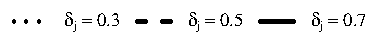
\includegraphics{LegendMarginal}

 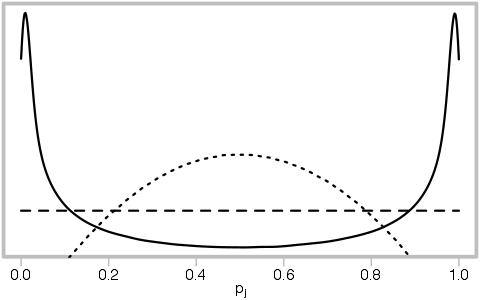
\includegraphics[width= 0.55\textwidth]{Marginals}
   \caption{The marginal distribution of $p_i$ under different levels of 
$\delta_i$.  The more the forecaster knows, i.e. the higher $\delta_i$ is, 
the more the probability forecasts are concentrated around the extreme 
points 0 and~1.}
\label{marginals}
\end{figure}

\section{Probability Extremizing}
\label{extremizing}
This section introduces the oracular aggregator $p'$ under the Gaussian partial information model and uses it to understand extremizing of the probit opinion pool $\probit$. This particular averaging aggregator was chosen because a) $\probit$ is more reasonable than the simple average $\bar{p}$, and b) $\probit$ is very similar to the logarithmic opinion pool $\plog$ but results in cleaner analytic expressions. The analysis also serves as an illustration on how the oracular aggregator can be used to analyze the behavior or expected performance of any aggregation technique -- and not just probability extremizing. 

\subsection{General Information Structure}
%We show that, under two specific Gaussian partial 
%information models, the oracle, on average,
%extremizes the probit aggregator. 
Recall from Section \ref{PIFintro} that the oracular aggregate is the conditional expectation of $\one_A$ given all the information of the forecasters. Under the Gaussian partial information model, this can be emulated by introducing an oracle forecaster whose information set is $I' := \bigcup_{i=1}^N I_i$.
Appending this to the multivariate Gaussian distribution~(\ref{Nforecasters}) gives
\begin{align}
\left(\begin{matrix} X_S \\ X_{I'} \\ X_{I_1}\\ \vdots \\ X_{I_N} 
 \end{matrix}\right) &\sim \mathcal{N}\left( 
 \boldsymbol{0}, 
% \left(\begin{matrix} 
%\Sigma_{11}' & \Sigma_{12}'\\
%\Sigma_{21}' & \Sigma_{22}\\
% \end{matrix}\right) 
% =
% 
 \left(\begin{array}{c c| c c cc }
1 & \delta' & \delta_1 & \delta_2 & \dots & \delta_N  \\ 
\delta' & \delta' & \delta_1 & \delta_2 & \dots & \delta_N  \\ \hline
\delta_1& \delta_1 & \delta_1 &\rho_{1,2} & \dots & \rho_{1,N}   \\ 
\delta_2 & \delta_2 &\rho_{2,1} & \delta_2 & \dots & \rho_{2,N}  \\ 
\vdots &\vdots & \vdots & \vdots & \ddots & \vdots  \\ 
\delta_N &\delta_N & \rho_{N,1} & \rho_{N,2} & \dots & \delta_N\\ 
 \end{array}\right)\right), \label{oracleN} 
\end{align}
where  $X_{I'}$  is the information known by the oracle and $\delta' = |I'|$ is the amount of this information.  Therefore, 
 \begin{align*}
p' = \P(X_S > 0 |  \mathcal{F}') 
   &= \Phi\left( \frac{X_{I'}}{\sqrt{1-\delta'}} \right)
\end{align*}

Given that, under the Gaussian partial information model, it is not possible to do better than $p'$, the oracular aggregator provides a benchmark for quantifying how much extremizing should be performed under any given circumstances. In particular, we say that a probability $p$ is extremized by another probability $q$ 
if and only if $q$ is closer to $0$ when $p \leq 0.5$ and closer 
to $1$ when $p \geq 0.5$.  Define the {\em probit extremization ratio}
to be the real number $\alpha(q,p) := \Phi^{-1}(q) / \Phi^{-1} (p)$. Therefore
$q$ extremizes $p$ when $\alpha(q,p) > 1$.  In the case where $p = \probit$ and $q = p'$,
the probit extremization ratio becomes
\begin{align}
\alpha(p', \probit)  = \frac{P_{I'}}{\frac{1}{N}\sum_{i=1}^N P_{I_i}}\label{alpha}
\end{align}
Unless otherwise stated, we denote (\ref{alpha}) simply with $\alpha$. This is a random quantity that spans the entire real line; that is, 
it is possible to find a set of probability forecasts and a distribution 
of information for any possible value of $\alpha \in \mathbb{R}$. 
Evidently, extremizing is not guaranteed to always improve the 
probit opinion pool.  
To understand when extremizing is likely to be beneficial, 
it is necessary to derive the probability distribution of $\alpha$. 
First, given that 
\begin{align*}
P_{I'} &\sim \mathcal{N}\left(0, \sigma^2_{1} = 
  \frac{\delta'}{1-\delta'} \right)\\ \frac{1}{N}\sum_{i=1}^N P_{I_i} 
&\sim \mathcal{N}\left(0, \sigma^2_{2} =\frac{1}{N^2} 
  \left\{ \sum_{i=1}^N \frac{\delta_i}{1-\delta_i} 
  + 2 \sum_{i,j: i<j} \frac{\rho_{ij}}{\sqrt{(1-\delta_j)(1-\delta_i)}}
  \right\} \right),
\end{align*}
the amount of extremizing $\alpha$ is a ratio of two correlated 
Gaussian random variables.  The Pearson product-moment correlation 
coefficient for them is
\begin{align*}
\kappa  &= 
  \frac{ \sum_{i=1}^N \frac{\delta_i}{\sqrt{1-\delta_i}}}
  {\sqrt{\delta'  \left\{ \sum_{i=1}^N \frac{\delta_i}{1-\delta_i} + 2 
  \sum_{i,j: i<j} \frac{\rho_{ij}}{\sqrt{(1-\delta_j)(1-\delta_i)}}\right\}}}
  \; 
\end{align*}
It follows that $\alpha$ has a Cauchy distribution as long as 
$\sigma_1 \neq 1$, $\sigma_2 \neq 1$, or $\kappa \pm 1$ 
(see, e.g., \citealt{cedilnik2004distribution} for this 
well known result).  These conditions are very mild under 
the Gaussian partial information model.  For instance, if no forecaster 
knows as much as the oracle, the conditions are satisfied. 
Consequently, the probability density function of $\alpha$ is
\begin{align*}
f(\alpha | x_0, \gamma) &= \frac{1}{\pi} 
  \frac{\gamma}{(\alpha-x_0)^2+\gamma^2}, 
\end{align*}
where 
\begin{align*}
x_0 = \kappa \frac{\sigma_1}{\sigma_2} \hspace{0.2in} \mbox{ and } 
  \hspace{0.2in} \gamma &= \frac{\sigma_1}{\sigma_2} \sqrt{1-\kappa^2} \, .
\end{align*}
The parameter $x_0$ represents the location (the median and mode) and 
$\gamma$ specifies the scale (half the interquartile range) of the 
Cauchy distribution. This leads to the following proposition. 
The proof of this and other propositions are deferred to the Appendix.

\begin{proposition}
\label{positiveProbThm}
The law of the extremization ratio $\alpha$ is a Cauchy with 
parameters $x_0$ and $\gamma$, where the location parameter 
$x_0$ is at least~1, equality occurring only when $\delta_i = \delta'$ 
for all $i = 1, \dots, N$. Consequently, if $\delta_i \neq \delta'$ 
for some $i = 1, \dots, N$, then the probability that the probit 
opinion pool requires extremizing is $\P(\alpha > 1 | \Sigma_{22}, \delta')$
which is strictly greater than $1/2$. 
\end{proposition}
\noindent
This proposition shows that, on any non-trivial problem, a small
perturbation in the direction of extremizing is more likely to 
improve the probit opinion pool than to degrade it.  This partially 
explains why extremizing aggregators perform well on large sets of 
real-world prediction problems.  It may be unsurprising after the fact,
but the forecasting literature is still full of articles that perform 
probability averaging without extremizing.  The next two 
sections examine subcases in which more detailed computations of the oracular aggregator can be performed. This sheds light on extremization in many real-world forecasting settings.  

\subsection{Fully- and Non-Overlapping Information}
\label{disjoint}
This section examines two limiting scenarios: a) the forecasters share no information, and b) the forecasters share all their information. First, consider the latter case where all the information sets are the same, $I_{i} = I_j$ for all $i \neq j$. Consequently, all the probability forecasts $\{p_i : i = 1, \dots, N\}$ are the same, and the probit opinion pool, the oracular aggregator, and the revealed aggregator equal to this common probability forecast. Therefore no extremization is needed. Given that the oracular forecast varies smoothly over the space of  information structures, averaging techniques such as the probit opinion pool can be expected to work well when the forecasts are based on very similar sources of information. This result is supported by the fact that the classical measurement error framework, which essentially describes the forecasters as making numerous small mistakes while applying the same procedure to the same data (recall Section \ref{ss:measurement}), result in averaging-based aggregators. 
%
% our discussion in Section \ref{ss:measurement} about the micro-level explanation of the classical measurement error framework. 
% For instance, the forecasters may discuss the forecasting problem before making their separate predictions. 


Next, consider the second case, where the forecasters' information sets do not overlap,  $|I_{i} \cap I_{j}| = 0$ for all $i \neq j$. Such an information structure is likely to arise if a team of forecasters strategically decide to access and study disjoint sources of information. The resulting information structure $\Sigma_{22}$ 
is diagonal, and hence coherent if and only if $\sum_{j=1}^N \delta_j \leq 1$. 
In this situation the oracular aggregator and the revealed aggregators
coincide because $p_i$ determines $X_i$ and $X_{I'}$ is the sum of
all the $X_i$. That is,
%Given that under non-overlapping information 
%$\delta' = \sum_{j=1}^N \delta_j$ and $X_{I'} = \sum_{j=1}^N X_{I_j}$, 
 \begin{align*}
p' &= p'' =  \Phi\left( \frac{\sum_{i=1}^N X_{I_i}}
  {\sqrt{1- \sum_{i=1}^N \delta_i}} \right) 
\end{align*}
This aggregator can be described in two steps: The first step consists of voting, or range voting to be more specific (see, e.g., \citealt{fishkin1997voice}), where the votes are weighted according to the importance of the forecasters' private information. This is performed by the summation in the numerator. If this sum falls below $0.0$ (or above $0.0$), the consensus believes that the event will not happen (or will happen). The second step is performed by the denominator that extremizes the  consensus according to the total amount of information in the group. For instance, if the forecasters know all the information, i.e. $\sum_{j=1}^N \delta_j = 1$, their vote deterministically indicates whether the event $A$ happens or not. This technique clearly leads to very extreme aggregate forecasts. Therefore more extreme techniques, such as voting, can be expected to work well if the forecasters use very different information sets.

%Combining this with our earlier discussion leads to the following observation.
In summary, the analysis suggests a spectrum of aggregators indexed by the 
information overlap.  The optimal 
aggregator undergoes a smooth transformation from 
averaging to summing of the probit forecasts as the information 
overlap decreases from full overlap towards the point of no overlap.
%This is summarized in the following observation.
%%\begin{observation}
%The information structures index a spectrum of aggregators. 
That is,
\begin{center}
\begin{tabular}{ccc}
%\stackrel{\text{ \normalsize full information overlap}}{\stackrel{\text{\normalsize no extremization}}{averaging}} && \Leftrightarrow  && \stackrel{\text{ no information overlap}}{\text{full extremization}}
%high information overlap & \multirow{2}{*}{$\Leftrightarrow$} & low information overlap\\
high information overlap & & low information overlap\\
low extremization & {\Large $\Longleftrightarrow$} & high extremization \\
averaging  & & voting\\
\end{tabular}
\end{center}
%\end{observation}
This observation gives qualitative
guidance in real world settings where the general level of overlap 
can said to be high or low.  For instance, forecasts from a group 
of forecasters working together or in close collaboration can be 
averaged while forecasts from a diverse group of forecasters working 
independently of each other should be aggregated via more extreme 
techniques such as voting (see \citealt{parunak2013characterizing} 
for a discussion on aggregation via voting). This spectrum is particularly visible in the next section that  examines the intermediate scenarios with partial information sharing among the forecasters.

%Because $p_i$ and $X_{I_i}$ are related by the one-to-one 
%transformation~(\ref{Indiv}), we may also write this as
% \begin{align}
%p' &= \Phi \left \{ \frac{1}{\sqrt{1 - \sum_{i=1}^N \delta_i}}
%   \; \sum_{i=1}^N \sqrt{1 - \delta_i} \Phi^{-1} (p_i) \right \} \, .
%\end{align}
%In the appendix we prove the following result.  Note that this 
%result is not distributional, it holds samplewise when all the
%forecasts fall on the same side of $1/2$.
%
%\begin{proposition}
%\label{positiveThmVote}
%Under the non-overlapping information structure, the extremization
%parameter $\alpha$ is at least $1$ either if every $X_{I_i} \geq 0$ 
%or if every $X_{I_i} \leq 0$ (equivalently, if every $p_i \geq 1/2$ 
%or every $p_i \leq 1/2$).
%\end{proposition}

\subsection{Partially Overlapping Information}
\label{compound}

%Assume that the forecasters' information sets have the 
%same size and that the amount of overlap between any two information 
%sets is constant, i.e., $|I_{1}| =  \dots = |I_{N}|$ and 
%$|I_{i} \cap I_{j}| = |I_{h} \cap I_{k}|$ for all $i \neq j$ 
%and $h \neq k$.  In this case the revealed aggregator is not
%as good as the oracular aggregator (the former is a conditional
%expectation of the latter).  
%%Here, we compare $\probit$ to the
%%oracular aggregator; in Section~\ref{compound2}
%%we compare the revealed aggregator to the probit opinion pool.
%The information structure $\Sigma_{22}$ is compound symmetric.  
%This structure would hold, for example, if the forecasters 
%sample information sources from a common distribution. 
%Assuming compound symmetric information in (\ref{oracleN}) results in
%\begin{align}
%\label{eq:symmetric}
%\left(\begin{matrix} X_{S} \\ X_{I'}\\ X_{I_1}\\ \vdots \\ X_{I_N} 
%   \end{matrix}\right) 
%  &\sim \mathcal{N}\left( \boldsymbol{0}, \left(\begin{matrix} 
%\Sigma_{11}' & \Sigma_{12}'\\
%\Sigma_{21}' & \Sigma_{22}\\
% \end{matrix}\right) 
% =
% \left(\begin{array}{cc|cccc}
%1 & \delta'& \delta & \delta & \dots & \delta  \\ 
%\delta' & \delta' & \delta & \delta & \dots & \delta  \\ \hline
%\delta & \delta &\delta & \lambda\delta & \dots & \lambda\delta   \\ 
%\delta& \delta & \lambda\delta & \delta & \dots & \lambda\delta  \\ 
%\vdots &\vdots & \vdots & \vdots & \ddots & \vdots  \\ 
%\delta &\delta & \lambda\delta & \lambda\delta & \dots & \delta\\ 
% \end{array}\right)\right)
%\end{align}
%
%The amount of information known by each forecaster is denoted 
%by $\delta \in [0,1]$.  The value of $\lambda$ is the proportion 
%of the information known to one forecaster that is also known to
%another single forecaster.  This minor change of parametrization 
%was made for the sake of simplifying some of the following expressions. 
%To ensure that $\Sigma_{22}$ is coherent, a restriction must 
%be placed on $\lambda$. 
%First, given that under any combination of $\delta$ and $N$ all forecasters 
%may know the exact same information, the value of $\lambda$ is 
%bounded from above by $1$. Second, observe that information overlap 
%is unavoidable when $\delta > 1/N$.  The minimum sharing occurs when 
%all information is either shared or private.  In other words, 
%if $\delta > 1/N$ and $I_{i} \cap I_j = I$ with $|I| =  \lambda \delta$ 
%for all $i \neq j$, the value of $\lambda$ is minimized when 
%$\lambda\delta + N(\delta - \delta\lambda) = 1$.  Therefore the 
%lower bound for $\lambda$ is $\max \left\{ \frac{N-\delta^{-1}}{N-1}, 
%0\right\}$, and $\Sigma_{22}$ is coherent if and only if
%\begin{align}
%\delta \in [0,1] &&  \lambda &\in \left[  
%   \max \left\{ \frac{N-\delta^{-1}}{N-1}, 0\right\}, 1 \right), 
%   \label{rhoDomain}
%\end{align}
%where the strict upper bound on $\lambda$ ensures that
%$\Sigma_{22}$ is not singular.  In the following discussion, 
%however, this technical restriction is ignored and the case 
%$\lambda = 1$ is analyzed as a limiting case.
%Plugging these simplifications in (\ref{alpha}) gives 
%\begin{align*}
%\alpha &= \frac{X_{I'}}{\frac{1}{N}\sum_{j=1}^N X_{I_j}} 
%  \sqrt{\frac{1-\delta}{1-\delta'}} 
%\end{align*}
%This follows a $\text{Cauchy}(x_0, \gamma)$ distribution with
%\begin{align*}
%x_0 &= \frac{N}{1+(N-1)\lambda}  \sqrt{\frac{1-\delta}{1-\delta'}}\\[2ex]
%  \gamma &=  \sqrt{\frac{N(\delta' + \delta' \lambda (N-1) - \delta N)}
%  {\delta (\lambda (N-1) + 1)^2}}\sqrt{\frac{1-\delta}{1-\delta'}}
%\end{align*}
The total amount of information among the forecasters $\delta'$ is uniquely determined by $\Sigma_{22}$ only when the group involves two forecasters. More specifically, $\delta' = \delta_1 + \delta_2 - \rho_{12}$ when $N=2$. By further assuming that $\delta = \delta_1 = \delta_2$, both $x_0$ and $\gamma$ depend only on two parameters and hence can be analyzed graphically. The results remain qualitatively similar even without assuming $\delta_1 = \delta_2$. This assumption, however, leads to fewer plots with essentially no loss of information. Let $\rho_{12} = \lambda\delta$, where the value of $\lambda$ is the proportion  of the information known to one forecaster that is also known to the other forecaster. Under these assumptions the information structure $\Sigma_{22}$ is coherent  if and only if
\begin{align*}
\delta \in [0,1] &&  \lambda &\in \left[  
   \max \left\{ 2-\delta^{-1}, 0\right\}, 1 \right] 
\end{align*}
%  When $N=2$, the information structure is coherent if and only if 
%\begin{align}
% \delta_1, \delta_2 \in [0,1] && \rho_{12} \in \left[  \max \left\{\delta_1+\delta_2 - 1,  0\right\}, \min \left\{\delta_1, \delta_2 \right\} \right] \nonumber
%\end{align}
%The analysis is almost fully general because compound symmetry under $N = 2$ forecasters is equivalent to only assuming $\delta_1 = \delta_2$. 


\begin{figure}[t]
\hspace{-1.2em}
    \centering
    \begin{subfigure}[b]{0.33\textwidth}
        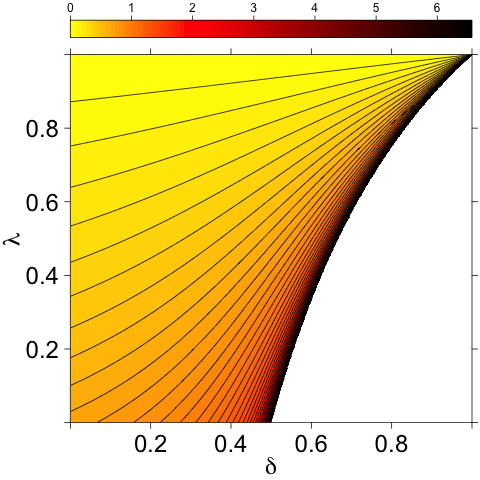
\includegraphics[width=1.07\textwidth, height = \textwidth]{ExtremeX0}
\caption{$\log(x_0)$}	
\label{xOracle}
    \end{subfigure}%
\hspace{0.6em}
    \begin{subfigure}[b]{0.33\textwidth}
        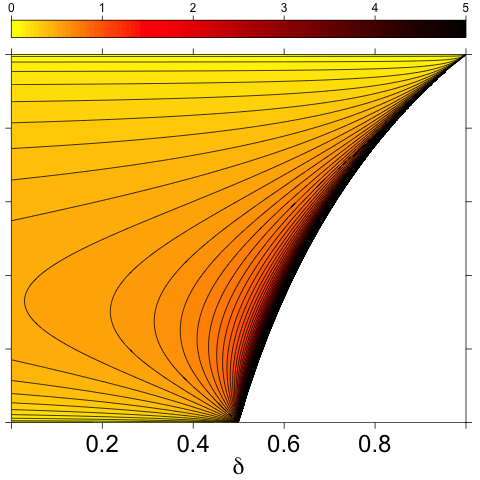
\includegraphics[width= 0.95\textwidth, height = \textwidth]{ExtremeGamma}
\caption{$\gamma$}
\label{gammaOracle}
        \end{subfigure}
\hspace{-1.3em}
    \begin{subfigure}[b]{0.33\textwidth}
        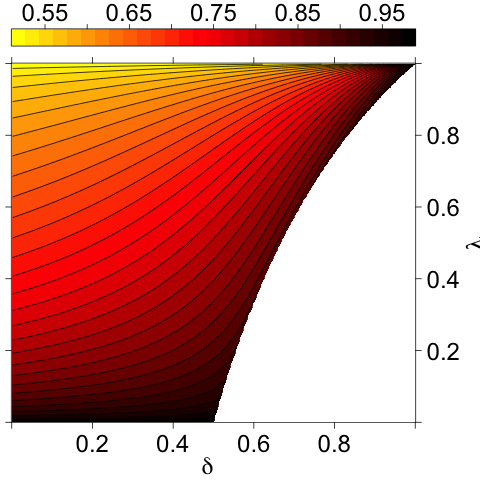
\includegraphics[width=1.07\textwidth, height = \textwidth]{Probs}
\caption{$\P(\alpha > 1 | \Sigma_{22}, \delta')$}
\label{probOracle}
        \end{subfigure}

    \caption{ The amount of extremizing follows a 
Cauchy$(x_0, \gamma)$, where $x_0$ is a location parameter and $\gamma$ 
is a scale parameter.  This figure considers only $N = 2$ forecasters.}
        \label{LevelplotsOracle}
\end{figure}
 
Figure \ref{LevelplotsOracle} shows $\log(x_0)$, $\gamma$, and $\P(\alpha > 1 | \Sigma_{22}, \delta')$ under all plausible combinations of $\delta$ and $\lambda$. High values have been censored to keep the scale manageable. Notice that extremizing is required 
more often when $\delta$ is high and $\lambda$ is low.  Given that 
$\delta'$ increases in $\delta$ but decreases in $\lambda$, the amount 
of extremizing can be expected to increase in the total amount of 
information among the forecasters $\delta'$.  This, however, does not 
provide a full explanation of extremizing.  Information diversity 
is also an important yet separate determinant of extremizing.  
To see this, observe that fixing $\delta'$ to some constant 
defines a curve $\lambda = 2 - \delta'/\delta$ on the plots in 
Figure~\ref{LevelplotsOracle}.  For instance, letting $\delta' = 1$ 
gives the boundary curve on the right side of each plot.  This curve 
then shifts inwards and rotates slightly counterclockwise as 
$\delta'$ decreases.  At the top end of each curve all forecasters 
know and share the total information, i.e. $\delta = \delta'$ and 
$\lambda = 1.0$.  At the bottom end, on the other hand, the forecasters 
partition the total information, i.e. $\delta = \delta'/2$, and 
share nothing, i.e. $\lambda = 0.0$.  Given that moving down along 
the curve increases both information diversity and the modal amount 
of extremizing, information diversity is an important determinant 
of extremizing together with the group's total amount of information.  
%This provides the basis for our second observation.
%\begin{observation}
Therefore extremization can be expected to increase in factors such as number of forecasters, subject-matter expertise, and human diversity, but to decrease in collaboration, sharing of resources, and problem difficulty.
%\begin{center}
%\begin{tabular}{l | l}
%increase in & decrease in\\ \hline
%Number of forecasters & Collaboration\\
%Subject-Matter forecasterise & Sharing of Resources\\
%Human Diversity & Problem Difficulty
%\end{tabular}
%\end{center}
%\end{observation}

%Therefore the amount of extremizing can be expected to increase 
%in many factors such as human diversity, subject-matter forecasterise, 
%and the extent to which forecasters can access information, but decrease 
%through forecaster collaboration and sharing of resources. 




\section{Probability Aggregation}
\label{aggregation}

This section first derives the revealed aggregator $p''$ for 
the general Gaussian partial information model. By assuming exchangeability among the forecasts, the revealed aggregator can be applied to any single pool of probabilities. After proving some properties of the revealed aggregator under exchangeability, it is tested on real-world forecasts. This a) illustrates one approach to estimating the information structures in practice, and b) provides some empirical evidence in favor of the partial information model. 
% We then apply 
%this to the symmetric case, for which the oracular aggregator 
%was discussed in Section~\ref{compound}.  The revealed aggregator, 
%unlike the oracular aggregator, can be applied in practice.  
%We prove an extremizing result for this aggregator.

\subsection{Revealed Aggregator for the Gaussian Model}

Referring back to (\ref{Nforecasters}), if $\boldsymbol{X} = 
(X_{I_1}, X_{I_2},  \dots, X_{I_N})'$ is a column vector 
of length $N$ and $\Sigma_{22}$ is a coherent overlap structure 
such that $\Sigma_{22}^{-1}$ exists, then 
\begin{align*}
X_{S} | \boldsymbol{X} \sim \mathcal{N}\left(\bar{\mu}, \bar{\Sigma}\right), 
\end{align*}
where
\begin{align*}
\bar{\mu} &= \mu_1 + \Sigma_{12} \Sigma_{22}^{-1} 
  (\boldsymbol{X} - \boldsymbol{\mu}_2) 
  = \Sigma_{12} \Sigma_{22}^{-1} \boldsymbol{X} \\
 \bar{\Sigma}&= \Sigma_{11} - \Sigma_{12} \Sigma_{22}^{-1} \Sigma_{21} 
 = 1 - \Sigma_{12} \Sigma_{22}^{-1} \Sigma_{21}   \, .
\end{align*}
These expressions can be found directly from the formulas for
the conditional multivariate Gaussian distribution (see, 
e.g.,~\citealt[Result~5.2.10, page~156]{ravishanker2001first}). 
This then leads to a probability aggregator that depends on 
$\Sigma_{22}$.  More specifically, the revealed aggregator is
\begin{eqnarray}
p'' & = & \P\left(A  | \boldsymbol{X}\right)  \nonumber \\
%%%& = & \P\left(X_{S} > 0 | \boldsymbol{X}\right) \nonumber \\
%&=& \Phi\left( \frac{\Sigma_{12} \Sigma_{22}^{-1} \boldsymbol{X} - \Phi^{-1}(1-\tilde{p})}
%   {\sqrt{1 - \Sigma_{12} \Sigma_{22}^{-1} \Sigma_{21}}}\right) 
&=& \Phi\left( \frac{\Sigma_{12} \Sigma_{22}^{-1} \boldsymbol{X}}
   {\sqrt{1 - \Sigma_{12} \Sigma_{22}^{-1} \Sigma_{21}}}\right) 
\label{GeneralAggregator} \, .
\end{eqnarray}
%Furthermore, if $\one_N$ is a column vector of ones and 
%$\boldsymbol{P} = (P_{I_1}, P_{I_2}, \dots, P_{I_N})'$, 
%then the extremization parameter for $p''$ with respect to
%$\probit$ is given by 
%\begin{align*}
%\alpha  &= \frac{N \Sigma_{12} \Sigma_{22}^{-1} 
%  \boldsymbol{X}}{\left(\boldsymbol{1}_N' \boldsymbol{P} \right) 
%  \sqrt{1 - \Sigma_{12} \Sigma_{22}^{-1} \Sigma_{21}}}  \, .
%\end{align*}
% where $\tilde{p} = \P(A)$ is the prior probability discussed in Section \ref{prelim} and 
 where $\boldsymbol{X} = \Phi^{-1}(\boldsymbol{p})\sqrt{1-\Sigma_{12}}$. To make practical use of this computation, we need values
for the entries of $\Sigma_{22}$.  As discussed in 
Remark (\ref{item:specific}) in Section~\ref{ss:Gaussian},
this may be done in one of three ways: by assumption, 
by estimation, or in a Bayesian manner. If one is to assume a structure, the most natural and non-informative
choice is the symmetric one. This is the topic in the following subsections.


%\section{Version 1}
\subsection{Aggregation under Symmetric Information}
\label{compound2}
%In this section we assume symmetry, meaning that ${\bf X}$ and
%$\Sigma$ are given by~\eqref{eq:symmetric}.  This assumption
%on the parameters of the model corresponds to
This section assumes a type of exchangeability
 among the forecasters.  While this is somewhat idealized,
it is a reasonable choice in a low-information environment where there is no historical or self-report data to
distinguish the forecasters.  The averaging aggregators described in 
Section~\ref{sec:prior}, for instance, are symmetric. Therefore,
to the extent that they reflect an underlying model, the model 
assumes exchangeability.

Under the Gaussian partial information model, this implies that the forecasters' information sets have the 
same size and that the amount of overlap between any two information 
sets is constant, i.e., $|I_{1}| =  \dots = |I_{N}|$ and 
$|I_{i} \cap I_{j}| = |I_{h} \cap I_{k}|$ for all $i \neq j$ 
and $h \neq k$.   
%Here, we compare $\probit$ to the
%oracular aggregator; in Section~\ref{compound2}
%we compare the revealed aggregator to the probit opinion pool.
The information structure $\Sigma_{22}$ is called \textit{compound symmetric}.  
This structure would hold, for example, if the forecasters sample information sources from a common distribution.
Plugging this structure in (\ref{oracleN}) gives
\begin{align*}
%\label{eq:symmetric}
\left(\begin{matrix} X_{S} \\ X_{I_1}\\ \vdots \\ X_{I_N} 
   \end{matrix}\right) 
  &\sim \mathcal{N}\left( \boldsymbol{0}, \left(\begin{matrix} 
\Sigma_{11} & \Sigma_{12}\\
\Sigma_{21} & \Sigma_{22}\\
 \end{matrix}\right) 
 =
 \left(\begin{array}{c|cccc}
1 & \delta & \delta & \dots & \delta  \\ \hline
%\delta' & \delta' & \delta & \delta & \dots & \delta  \\ \hline
\delta  &\delta & \lambda\delta & \dots & \lambda\delta   \\ 
\delta & \lambda\delta & \delta & \dots & \lambda\delta  \\ 
\vdots & \vdots & \vdots & \ddots & \vdots  \\ 
\delta  & \lambda\delta & \lambda\delta & \dots & \delta\\ 
 \end{array}\right)\right),
\end{align*}
where the amount of information known by a forecaster is  $\delta \in [0,1]$, and the value of $\lambda$ is the proportion 
of information known to one forecaster that is also known to
another single forecaster.  
%This minor change of parametrization 
%was made for the sake of simplifying some of the following expressions. 
To ensure that $\Sigma_{22}$ is coherent, a restriction must 
be placed on $\lambda$. 
First, given that under any combination of $\delta$ and $N$ all forecasters 
may know the exact same information, the value of $\lambda$ is 
bounded from above by $1$. Second, observe that information overlap 
is unavoidable when $\delta > 1/N$.  The minimum sharing occurs when 
all information is either shared with everyone or private to a single forecaster.  In other words, 
if $\delta > 1/N$ and $I_{i} \cap I_j = I$ with $|I| =  \lambda \delta$ 
for all $i \neq j$, the value of $\lambda$ is minimized when 
$\lambda\delta + N(\delta - \delta\lambda) = 1$.  Therefore the 
lower bound for $\lambda$ is $\max \left\{ \frac{N-\delta^{-1}}{N-1}, 
0\right\}$, and $\Sigma_{22}$ is coherent if and only if
\begin{align}
\delta \in [0,1] &&  \lambda &\in \left[  
   \max \left\{ \frac{N-\delta^{-1}}{N-1}, 0\right\}, 1 \right), 
   \label{rhoDomain}
\end{align}
where the strict upper bound on $\lambda$ ensures that
$\Sigma_{22}$ is not singular.  
%In the following discussion, 
%however, this technical restriction is ignored and the case 
%$\lambda = 1$ is analyzed as a limiting case.
%Plugging these simplifications in (\ref{alpha}) gives 
%\begin{align*}
%\alpha &= \frac{X_{I'}}{\frac{1}{N}\sum_{j=1}^N X_{I_j}} 
%  \sqrt{\frac{1-\delta}{1-\delta'}} 
%\end{align*}
%This follows a $\text{Cauchy}(x_0, \gamma)$ distribution with
%\begin{align*}
%x_0 &= \frac{N}{1+(N-1)\lambda}  \sqrt{\frac{1-\delta}{1-\delta'}}\\[2ex]
%  \gamma &=  \sqrt{\frac{N(\delta' + \delta' \lambda (N-1) - \delta N)}
%  {\delta (\lambda (N-1) + 1)^2}}\sqrt{\frac{1-\delta}{1-\delta'}}
%\end{align*}
Under this assumption, the general form of the revealed aggregator~(\ref{GeneralAggregator}) 
simplifies to
\begin{align}
p''
  &=\Phi\left(\frac{\frac{1}{(N-1)\lambda +1} 
  \sum_{i=1}^N X_{I_i} }{\sqrt{1- \frac{N\delta}{(N-1)\lambda +1} }}  
  \right) \, \label{CompoundAggre}
\end{align}
%Recall from section \ref{compound} that $\delta \in [0,1]$ can be 
%interpreted as the average amount of information known by an forecaster, 
%and $\lambda$ is the average proportion of the known information shared 
%between any two forecasters. 
The domain restriction (\ref{rhoDomain}) 
ensures that the term under the square-root in (\ref{CompoundAggre}) 
is always non-negative. In this case the revealed aggregator is not
as good as the oracular aggregator (the former is a conditional
expectation of the latter). 

Given these interpretations, it may at first seem surprising that 
the values of $\delta$ and $\lambda$ can be estimated in practice. 
Intuitively, the estimation relies on two key aspects of the model: 
a) the further the forecast is from the non-informative prior 
(typically at $0.5$), the more informed the forecaster is likely to be 
(see Figure~\ref{marginals}); and b) the more similar any two forecasts 
are, the more information overlap the corresponding forecasters are likely 
to have. This provides enough leverage to estimate the information structure   
via the maximum likelihood method.  Complete technical details and 
instructions for this are provided in the Appendix.  Besides exchangeability, 
the revealed aggregator (\ref{CompoundAggre}) is based on 
very different modeling assumptions than the averaging aggregators 
described in Section~\ref{sec:prior}. The following proposition summarizes some of the properties of the revealed aggregator (\ref{CompoundAggre}). 

\begin{proposition} \label{positiveThm}
Under symmetric information, 
\begin{enumerate}
\item[$(i)$] the probit extremization ratio between the revealed aggregator $p''$ and the probit opinion pool $\probit$ is given by the non-random quantity
\begin{align*}
\alpha(p'', \probit)
%&= \frac{\displaystyle{\frac{N\sqrt{1-\delta}}{(N-1)\lambda +1}}}
%  {\displaystyle{\sqrt{1- \frac{N\delta}{(N-1)\lambda +1} }}} 
 &=  \frac{\gamma \sqrt{1 - \delta}}{\sqrt{1-\delta\gamma}}
\end{align*}
where 
$$\gamma = \frac{N}{(N-1)\lambda +1},$$
\item[$(ii)$] the revealed aggregator $p''$ extremizes the probit opinion 
pool $\probit$ as long as $p_j \neq p_i$ for some $j \neq i$, and
\item[$(iii)$] the revealed aggregator $p''$ can leave the convex hull of the 
individual probability forecasts. 
\end{enumerate}
\end{proposition}
This proposition suggest that the revealed aggregator (\ref{CompoundAggre}) is appropriate 
for combining probability forecasts. To test this claim, the next subsection applies it to a set of real-world forecasts. The aggregation is done one problem at a time without assuming any other information besides the probability forecasts themselves. That is, the outcomes of the events are not known. This way any performance improvements reflect better fit of the underlying model. 



%This is a non-random quantity that depends only on three 
%parameters.  Therefore it can be conveniently analyzed graphically. 
%Figure~\ref{Levelplots} considers $N = 2$ and $N = 10$ forecasters, 
%and describes the amount of log-extremizing $\log(\alpha)$ under 
%all plausible combinations of $\lambda$ and $\delta$.  High values 
%have been censored to keep the scale manageable.  Even though the 
%patterns in Figure \ref{Levelplots} are very similar to the ones 
%shown earlier in Figure~\ref{LevelplotsOracle}, comparing 
%$\alpha$ under $N = 2$ and $N = 10$ leads to new observations. 
%First, holding both $\delta$ and $\lambda$ fixed, the amount of 
%extremizing $\alpha$ increases in $N$.  This can be considered as 
%being caused by an increase in the total amount of information 
%among the forecasters because $\delta'$ increases in $N$.  Second, 
%in general, having many forecasters, each with a considerable amount 
%of information, simply leads to unavoidable information overlap. 
%This is illustrated in Figure~\ref{Levelplots} where the set of 
%possible values of $\lambda$ decreases very rapidly as $\delta$ 
%increases. Furthermore, moving from Figure~\ref{ExtremeN2} to 
%Figure \ref{ExtremeN10} illustrates how the dependence between 
%$\lambda$ and $\delta$ strengthens as $N$ increases.  In fact, 
%based on the domain restriction (\ref{rhoDomain}), the value of 
%$\lambda \to 1$ as $N \to \infty$ under any given $\delta$. 
%Therefore in the limit the group of forecasters is equivalent to 
%a single forecaster.  The compound symmetric information structure, 
%however, is almost fully general when $N = 2$.  Therefore assuming 
%compound symmetric information can be appropriate for small numbers 
%of forecasters but becomes restrictive as more forecasters enter the group. 
%
%\begin{figure}[ht!]
%\centering
%\hspace*{1.2em} 	
%\includegraphics[width=0.973\textwidth, height = 3em]{colorkey} 
%    \centering
%    \begin{subfigure}[b]{0.499\textwidth}
%        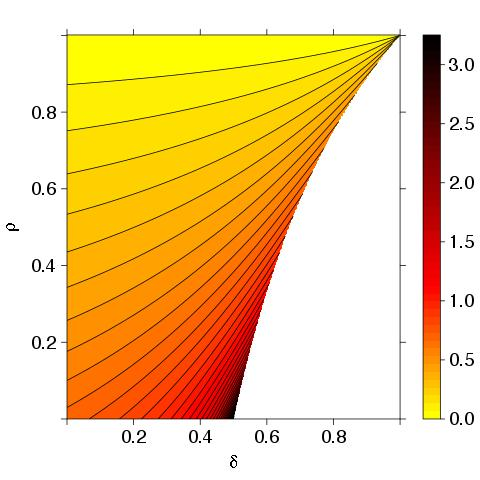
\includegraphics[width=\textwidth]{ExtremeN2}
%\caption{N = 2}	
%\label{ExtremeN2}
%    \end{subfigure}%
%    \begin{subfigure}[b]{0.499\textwidth}
%        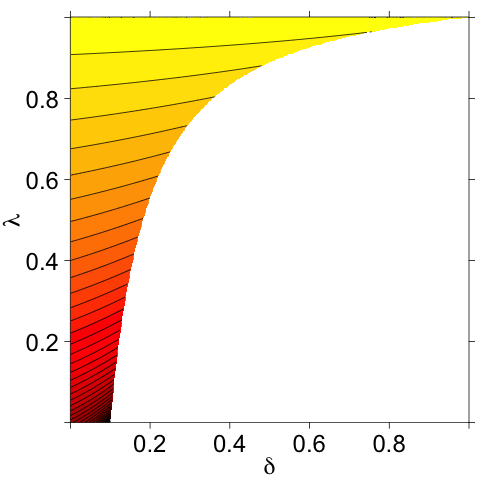
\includegraphics[width=\textwidth]{ExtremeN10}
%\caption{N = 10}
%\label{ExtremeN10}
%    \end{subfigure}
%    \caption{ The amount of log-extremizing $\log(\alpha)$ under 
%    different combinations of $N$ (the number of forecasters), 
%    $\delta$ (the average amount known by one forecaster), and 
%    $\lambda$ (the average amount shared by any two forecasters).}
%    \label{Levelplots}
%\end{figure}
%\clearpage

\subsection{Real-World Forecasting Data}
\label{realData}
The Good Judgment Project (GJP) (see, e.g., \citealt{mellers2014psychological, ungar2012good}) is 
a research study that started in 2011 and has ever since recruited thousands of forecasters 
from professional societies, research centers, and alumni associations. 
These forecasters face questions about future international 
political events, estimate the probability of each event, and 
update their predictions when they feel the probabilities have changed.  
The forecasters know that their probability estimates are assessed 
for accuracy using Brier scores. 
% This incentivizes 
%the forecasters to report their true beliefs instead of attempting 
%to game the system (\citealt{winkler1968good}). 
 In addition to receiving 
\$150 for meeting minimum participation requirements that do not depend 
on prediction accuracy, the forecasters receive status rewards for 
their performance via leader-boards displaying Brier scores for the 
top 20 forecasters.  Every year the top 2\% percent of the forecasters 
are selected to the elite group of ``super-forecasters''.  
%The 
%super-forecasters work in groups to make highly accurate predictions 
%on the same events as the rest of the forecasters. 

This section illustrates the revealed aggregator (\ref{CompoundAggre}) on forecasts made by the super-forecasters. These forecasters were chosen to the group of super-forecasters during the first year of the GJP. Our evaluation, however, only uses forecasts that were made during the second year. Therefore, the individual forecasts are likely, but not guaranteed, to be good. This group of super-forecasters consisted of 44 forecasters making predictions about 123 geopolitical events with two possible outcomes. For instance, some of the questions were
\begin{quote}\textit{
Will France withdraw at least 500 troops from Mali before 10 April 2013?
}\end{quote}
and
\begin{quote}\textit{
Will a banking union be approved in the EU council before 1 March 2013? 
}
\end{quote}
 The forecasters were allowed to update their forecasts as long as the questions were active. Some questions were active longer than others. In fact, the number of active days ranged from 3 to 284 days, with a mean of 96 days. This paper, however, does not focus on dynamic data. For this reason, we only consider the each forecaster's most recent forecasts in the first three days of a problem because this is when most uncertainty is present. 
% the first three days for each problem because this is when the most of uncertainty is present. If a super-forecaster made more than one forecast within these three days, only the most recent forecast is considered. Only super-forecasters who made at least one forecast within the these days were considered  as participants for that particular problem. 
In the resulting dataset, the number of forecasts per event ranged from 17 to 34 forecasts, with a mean of 24.2 forecasts. To avoid infinite log-odds and probit scores, extreme forecasts $p_i = 0$ and $1$ have been censored to $p_i = 0.001$ and $0.999$, respectively.
 
 
The results are presented in terms of the mean Brier scores (BS), i.e. the quadratic loss. To make this more concrete, consider $K$ problems and let $p_k$ be the aggregate forecast for the event $Y_k$, where $k = 1, \dots, K$. Then,
 \begin{align*}
BS &= \frac{1}{K} \sum_{k=1}^K (p_k - Y_k)^2
 \end{align*}
 This score can be decomposed into three parts: reliability (REL), resolution (RES), and uncertainty (UNC). The decomposition assumes that the aggregate forecast can only take discrete values $f_j \in [0,1]$ with $j = 1, \dots, J$. Let $n_j$ be the number of times $f_j$ occurs, and denote the empirical frequency of the corresponding events with $o_j$.  Let $\bar{o}$ be the overall empirical frequency of occurrence, i.e. $\bar{o} = \frac{1}{K} \sum_{k=1}^K Y_k$. Then the mean Brier score decomposes into 
 \begin{align*}
BS &= REL - RES + UNC\\
&= \frac{1}{K} \sum_{j=1}^J n_j (f_j - o_j)^2 - \frac{1}{K} \sum_{j=1}^J n_j (o_j - \bar{o})^2 + \bar{o}(1-\bar{o})
 \end{align*}
 Small values of the reliability term suggest improved calibration. The resolution term, on the other hand, describes how far the aggregate forecasts are from the naive forecast given by the average $\bar{o}$. The typical goal is to seek for an aggregate forecast that maximizes resolution subject to being calibrated (see, e.g., \citealt{gneiting2007probabilistic}). The uncertainty term quantifies overall uncertainty among the events and does not depend on the aggregate forecasts. 
 
 % latex table generated in R 3.0.3 by xtable 1.7-3 package
% Tue Aug 26 11:03:33 2014
\begin{table}[t]
\centering
\begin{tabular}{rrrrr}
  \hline
Aggregator & BS & REL & RES & UNC \\ 
  \hline
$\bar{p}$ & 0.1306 & 0.0351 & 0.0565 & 0.1520 \\ 
 $\plog$ & 0.1246 & 0.0262 & 0.0536 & 0.1520 \\ 
 $\probit$ & 0.1241 & 0.0272 & 0.0551 & 0.1520 \\ 
 $p''$ & 0.1199 & 0.0198 & 0.0520 & 0.1520 \\ 
   \hline
\end{tabular}
\caption{The mean Brier scores (BS) with its three components, reliability (REL), resolution (RES), and uncertainty (UNC), for the aggregated super-forecasts.}
\label{BrierTable}
\end{table}

Table \ref{BrierTable} shows the Briers scores for the average forecast $\bar{p}$, logarithmic opinion pool $\plog$, probit opinion pool $\probit$, and the revealed aggregator under symmetric information $p''$. No empirical approaches were considered for two reasons: a) they do not reflect an actual model of forecasts, and b) they require a training set with known outcomes and hence cannot be applied to one-time events. As can be seen in Table \ref{BrierTable}, the average forecast is clearly the worst performing aggregator. As discussed earlier, the two opinion pools, $\probit$ and $\plog$, are very similar. Consequently, they present almost identical scores. Even though the revealed aggregator is the least resolved, it presents greatly improved calibration and, therefore, achieves the lowest Brier score among all the aggregators. This is certainly an encouraging result. It is important to note, however, that the revealed aggregator under the symmetric information is only the first attempt in partial information aggregation. More elaborate information structures and estimation procedures are very likely to lead to many further improvements. 

%\section{Version 2}
%
%\subsection{Empirical Analysis}
%Even though the partial information model can be used for aggregating $N$ forecasts, preliminary calculations suggest that ensuring a coherent overlap structure for $N$ experts requires $\mathcal{O}\left(2^N\right)$ of constraints. Therefore further assumptions are required in practice. One promising simplification assumes $\{I_j\}_{j=1}^N$ to be intervals instead of any Borel measurable sets (for more information see \citet{kobler2012interval}). For the sake of brevity, however, the development and analysis of such methodology is left for future work.  Instead, akin to many related studies such as \citet{Ranjan08} and \citet{Geo}, the focus here is on aggregation of forecasts from two experts participating on $K$ prediction problems. More specifically, the aggregators receive $K$ pairs of forecasts but not the outcomes of the corresponding events. The overlap structure has only three constraints and can be estimated without making further assumptions on the form (such as an interval) of the information sets $\{I_j\}_{j=1}^N$. Furthermore, this gives cleaner expressions and a more concise discussion of the main points. 
%
%This section compares $p''$ against $\probit$ with different amounts of extremizing. Following our earlier notation, $\probit$ that has been extremized by some amount $\alpha \geq 1$ equals 
%\begin{align*}
%\probit(\alpha) &= \Phi \left\{ \frac{\alpha}{2}  \left[ \Phi^{-1}(p_1) + \Phi^{-1}(p_2) \right] \right \}
%\end{align*}
%Therefore $\alpha = 1$ suggests no extremization, and $\probit(1)$ represents the usual probit opinion pool $\probit$. In this section the aggregator $\probit(\alpha)$ is evaluated at different fixed values of $\alpha$ as if the value of $\alpha$ was chosen before the experiment. Let $\alpha_{opt}$ represent the value of $\alpha$ that shows best performance. In practice finding this value requires the knowledge of the event outcomes. Given that the outcomes are not assumed known in this paper, the optimal aggregator $\probit(\alpha_{opt})$ provides a highly, if not even an unfairly, competitive benchmark. Outperforming this benchmark would certainly provide evidence in favor of the partial information model. 
%
%
%Before $p''$ can be applied to the forecasts, it is necessary to estimate the overlap structure. Ideally this overlap structure would be estimated within each separate problem. Unfortunately, this is difficult because each problem is associated with only two forecasts. Therefore, to make this estimation feasible, we assume that  the overlap structure does not change across problems. Under this assumption,  all $K$ pairs of forecasts can be used to estimate the overlap structure. The Appendix provides details on the estimation procedure. Given that this assumption is unlikely to hold in practice, it is necessary to understand how robust the revealed aggregator is to cross-problem variation in the information structure. This is analyzed in the next subsection. 
%
%\subsubsection{Simulation Study: Sensitivity to  Cross-Problem Variation}
%Sensitivity to changed in the overlap structure across problems can be examined by applying the aggregators to $K$ pairs of forecasts all drawn from the Gaussian partial information model but with different overlap structures. More specifically, the simulation first draws
%\begin{align*}
%\delta_1, \delta_2 &\sim \mathcal{U}(0,1)\\
%\rho_{12} | \delta_1, \delta_2 &\sim \mathcal{U}[\max(0,\delta_1+ \delta_2-1), \min(\delta_1, \delta_2)]
%\end{align*}
%% $\delta_1$ and $\delta_2$ uniformly at random from the interval $[0,1]$. Next the overlap parameter $\rho_{12}$ is  drawn uniformly at random from the interval $[\max(0,\delta_1+ \delta_2-1), \min(\delta_1, \delta_2)]$. 
%This ensures that the resulting overlap structure is coherent. Next two binary (column) vectors, $\boldsymbol{v}_1$ and $\boldsymbol{v}_2$, of length $L$ are constructed such that $\boldsymbol{v}_1'\boldsymbol{v}_1/L = \delta_1$, $\boldsymbol{v}_2'\boldsymbol{v}_2/L = \delta_2$, and $\boldsymbol{v}_1'\boldsymbol{v}_2/L = \rho_{12}$. These vectors represent discrete approximations of the experts' basic information. The expert, however, may know more (or less) than this about any individual problem. Therefore the overlap structure for the $k$th problem is given by $\boldsymbol{v}_{1,k}$ and $\boldsymbol{v}_{2,k}$ that are perturbed versions of $\boldsymbol{v}_1$ and $\boldsymbol{v}_2$. More specifically, for $j = 1, 2$ the vector $\boldsymbol{v}_{j,k}$ is constructed by randomly either increasing or decreasing the number of ones in $\boldsymbol{v}_j$ such that 
%%
%%by a percentage amount drawn uniformly from $[0, \Delta]$ for $j = 1,2$. Therefore 
%the largest possible difference between $\boldsymbol{v}_{j,k}'\boldsymbol{v}_{j,k}/L = \delta_{j,k}$ and $\delta_j$  is $\Delta/2$. Consequently, the maximum difference in the expert's amount of information between any two problems is $\Delta$. This provides the means for a broad yet realistic variation across problems.
%
%%from one problem to another is approximately $\Delta \%$. 
% 
% \begin{figure}[h!]
%    \centering
%    \vspace{-1em}
%    \begin{subfigure}[b]{\textwidth}
%\hspace{9em}        \includegraphics{PertLegend}
%\label{pert1}
%    \end{subfigure}%
%
%
%    \begin{subfigure}[b]{0.32\textwidth}
%        \includegraphics[width=\textwidth, height = \textwidth]{PertN30Delta0}
%\caption{$\Delta = 0.0$}	
%\label{pert1}
%    \end{subfigure}%
%    \begin{subfigure}[b]{0.32\textwidth}
%        \includegraphics[width=\textwidth, height = \textwidth]{PertN30Delta01}
%\caption{$\Delta = 0.2$}	
%\label{pert2}
%    \end{subfigure}%
%    \begin{subfigure}[b]{0.32\textwidth}
%        \includegraphics[width=\textwidth, height = \textwidth]{PertN30Delta05}
%\caption{$\Delta = 1.0$}	
%    \end{subfigure}%
%        
%    \caption{The Brier scores of $p''$ and $\probit(\alpha)$ under three levels of perturbation.}
%        \label{Perturbation}
%\end{figure}
%
%Figure \ref{Perturbation} shows the Brier scores under different levels of perturbation $\Delta$. In each case the simulation ran for a total of 10,000 iterations. During every such iteration the experts participated in $K = 30$ problems. Figure \ref{pert1} shows that the revealed aggregator $p''$ outperforms $\probit(\alpha_{opt})$ by a noticeable margin when there is no perturbation, i.e. $\Delta = 0.0$. This performance gap, however, closes as $\Delta$ approaches $0.2$. Figure \ref{pert2} shows the Brier scores when $\Delta = 0.2$. At this point the amount of information can change by $0.2$ from one problem to another, and $p''$ performs similarly to $\probit(\alpha_{opt})$. After this point $p''$ loses to the $\probit(\alpha_{opt})$ but not by too much. In fact, even when the amount of information can change by $1.0$ from one problem to another, $p''$ loses only by $0.002$. At the same time $p''$ outperforms $\probit$ by $0.005$. If the number of problems $K$ is increased from $30$ to $50$ or $100$, the value of $\Delta$ at which the performances of $p''$ and $\probit(\alpha_{opt})$ meet increases from $0.2$ to around $0.35$ and $0.45$, respectively. Therefore $p''$ is less sensitive to information variation under larger values of $K$. For the sake of brevity, these results are not presented here separately. 
% 
%This seemingly good robustness can be understood as follows: $p''$ uses the forecasts across many problems to estimate how the experts' information sets generally relate to each other. In our simulation, this relationship is defined by  $\delta_1$, $\delta_2$, and $\rho_{12}$. This information is enough for the revealed aggregator to achieve good performance on most of the problems. As $K$ increases, the revealed aggregator $p''$ can estimate the general information overlap with improved accuracy and hence present even higher robustness. 
%
%\subsubsection{Simulation Study: Preservation of Calibration}
%According to \citet{Ranjan08} all convex combinations of the forecasts are necessarily poorly calibrated even when the individual forecasts themselves are calibrated. Unfortunately, this includes most of the widely used aggregators. In fact, to our knowledge, no model-based aggregator to date has been shown to preserve calibration. The revealed aggregator $p''$, however, cannot be formulated as a convex combination of the individual forecasts. This motivates us to examine how $p''$ behaves at different levels of calibration among the individual forecasts. Given that assessing calibration requires knowledge of the outcomes of the events, without knowing the outcomes the best one can really hope is to have an aggregator that presents at least as good calibration as the individual forecasters. 
%
%
%Experts should make probability assessments that are as far from the baseline as possible. The extent to which their probabilities differ from the baseline is measured by \textit{sharpness} (\citet{gneiting2008rejoinder, winkler2008comments}). If the experts are both sharp and well-calibrated, they can forecast the behavior of the process with high certainty and accuracy. Therefore useful probability estimation should  maximize sharpness subject to calibration (see, e.g., \citet{raftery2005using, murphy1987general}). Typically the quality of a probability forecast is evaluated with a reliability plot that is a simple tool for visually assessing the sharpness and calibration of a forecaster. The idea is to plot the forecasted probabilities against the observed empirical frequencies. Therefore any deviation from the diagonal line suggests poor calibration. A forecaster is considered under-confident (or over-confident) if the points follow an S-shaped (or \reflectbox{S}-shaped) trend. To assess sharpness of the forecaster, it is common practice to place a histogram of the given forecasts in the corner of the plot. Given that the data were balanced, any deviation from the the baseline probability of 0.5 suggests improved sharpness. Figure \ref{ExpertTypes} shows the reliability plot of three types of forecasters: under confident, calibrated, and over confident. 
%
%
%%allows us to illustrate that $p''$ in fact preserves calibration rather well. A secondary goal in this subsection is to examine how sensitive the revealed aggregator is to poor calibration of the individual forecasts.
%
%%the main goal is to understand how well the revealed aggregator is calibrated if the individual forecasts are calibrated. 
%
%The choice of the model used for simulating the forecasts is generally subjective, and the best one can do is to generate forecasts from a distribution that is as general and non-informative as possible. Therefore, in this subsection, the forecasts are not generated from the partial information model but rather from a non-informative model based on the classical measurement error framework. This choice has been motivated by the reliability plots. First, recall that the classical measurement error framework typically assumes that the forecasts are independent given the truth. Therefore, to generate the forecasts for the $k$th problem, the outcome of the event $Y_k$ is first generated with $\P(Y_k = 1) = 0.5$. Conditional on this outcome, the forecasts are then drawn from
%\begin{align*}
%p_{jk} |Y_k &\stackrel{iid}{\sim} \begin{cases}
%2p_{jk}& \text{ if } Y_k = 1\\
%2(1-p_{jk})& \text{ if } Y_k = 0,
%\end{cases}
%\end{align*}
%for $j = 1, 2$ with $p_{jk} \in [0,1]$. This gives probability forecasts that are calibrated and follow marginally a uniform distribution. To introduce over- or underconfidence, we rotate the forecasts' density function about the point $(0.5, 1.0)$. The marginal distribution is kept uniform. See the Appendix for a detailed discussion on how such forecasts are sampled. We consider three types of forecasters: underconfident, calibrated, and overconfident. The reliability plots of these types are given in Figure \ref{ExpertTypes}. The calibration plots are rotated counter- or clockwise by around 6.8 degrees (0.1 radians) for the under- and overconfident forecasters, respectively. Observe that the underconfident forecaster does not make any extreme forecasts. In particular, the forecasts are bounded between $[0.175,0.825]$. 
% \begin{figure}[h!]
%    \centering
%    \begin{subfigure}[b]{0.32\textwidth}
%        \includegraphics[width=\textwidth, height = \textwidth]{UnderconfidentExpert.pdf}
%\caption{Underconfident}	
%\label{UE}
%    \end{subfigure}%
%    \begin{subfigure}[b]{0.32\textwidth}
%        \includegraphics[width=\textwidth, height = \textwidth]{CalibratedExpert.pdf}
%\caption{Calibrated}	
%\label{CE}
%    \end{subfigure}%
%    \begin{subfigure}[b]{0.32\textwidth}
%        \includegraphics[width=\textwidth, height = \textwidth]{OverconfidentExpert.pdf}
%\caption{Overconfident}	
%    \end{subfigure}%
%\label{OE}
%        
%    \caption{Three types of forecasters considered in this section.}
%        \label{ExpertTypes}
%\end{figure}
%%
%%
%%\begin{figure}[htbp]
%%   \centering
%%   \includegraphics[width = 25em]{BS_Ns} % requires the graphicx package
%%   \caption{The Brier scores of the revealed aggregator under different numbers of problems $K$ and the probit opinion pool under different amounts of extremizing $\alpha$}
%%   \label{CalibrationNs}
%%\end{figure}
%%\textcolor{red}{Explain reliability plots first before jumping into explaining how simulation is done etc. This is important to understand the generality of the model}\\
%
%
%%Figure \ref{CalibrationNs} show the Brier scores of $p''$ and $\probit$ under different amounts of extremizing. Similarly to the previous section, the amount of extremizing was not learned from a training set. Instead, it was treated fixed. As can be seen in Figure \ref{CalibrationNs} the performance of $p''$ approaches to the performance of the optimally extremized $\probit$ as $K$ grows large.  At the same time the calibration of $p''$ improves. Even at $K = 10$, however, the calibration of $p''$ is very good.
%
%Figure \ref{CalibrationPlots} which shows a $4 \times 3$ grid of reliability plots. The dimensions span the aggregators, $\probit$, $\probit(\alpha_{opt})$, $p''$ with $K = 10$, and $p''$ with $K = 100$, from top to bottom, respectively, and the type of forecasters used, underconfident, calibrated, and overconfident, from left to right, respectively.  To guide our assessment, the dashed bands around the diagonal connect the point-wise, Bonferroni-corrected (\citet{bonferroni}) 95\% lower and upper critical values under the null hypothesis of calibration. These have been computed by running the bootstrap technique described in \citet{brocker2007increasing} for 10,000 iterations. In each case both forecasters were of the same type. The simulation was run for a total of $10,000$ iterations. 
%
%As was predicted by \citet{Ranjan08} and seen in the top row for Figure \ref{CalibrationPlots}, $\probit$ is poorly calibrated and lacks sharpness,i.e. the aggregates are too close to $0.5$, under all types of forecasters. Based on the middle row, however, extremizing $\probit$ yields good calibration and improved sharpness except when the forecasters are overconfident. The optimal extremizing constant $\alpha_{opt}$ varies from $4.3$ (under confident) to $2.7$ (calibrated) and finally to $1.9$ (overconfident). Therefore no value of $\alpha$ is optimal for all types of forecasters. Instead, the optimal value $\alpha_{opt}$ must be learned from a training set on a case-by-case basis. 
%
%The bottom row of  \ref{CalibrationPlots} shows reliability plots for $p''$. The level of calibration of $p''$ seems to follow that of the individual forecasters' rather closely, hence obeying the dictum ''what you put in is what you get out.'' The revealed aggregator $p''$ with $K = 10$ presents slight overconfidence at extreme probabilities when the individual forecasters are calibrated.  The overconfidence, however, vanishes as $K$ becomes large. This can be understood as follows: when $K$ is small, an expert's forecast close to $0.0$ or $1.0$ suggests more strongly that the expert's information set is very large. Therefore an expert is likely to appear highly knowledgeable when $K$ is small rather than large. When either expert is deemed very knowledgeable, the aggregator follows and extremizes that expert's forecasts strongly. Given that the individual expert's forecasts are calibrated, extremizing them leads to overconfidence. Overall, however, the level of calibration remains stable through aggregation. In addition, the revealed aggregator is able to improve sharpness. This is present when the forecasters are under confident but particularly visible under calibrated and overconfident forecasters. 
%
%%In terms of Brier scores, the aggregate forecasts present better performance than the individual forecasters under all types of forecasters. Therefore aggregation is deemed beneficial. There are, however, noticeable differences among the aggregators. The extremizing aggregator $\probit(\alpha_{opt}$ performs the best under any type of forecaster. The revealed aggregator $p''$ is able to outperform $\probit$ when the forecasters are under confident or calibrated but not when they are overconfident. This is mostly due to the inherent under confidence of $\probit$. 
%
%
%\begin{figure}
%    \centering
%    \begin{subfigure}[b]{0.32\textwidth}
%        \includegraphics[width=\textwidth, height = \textwidth]{UnderconfidentProb10}
%%\caption{The forecasts made by expert 1}	
%\label{Expert1}
%    \end{subfigure}%
%    \begin{subfigure}[b]{0.32\textwidth}
%        \includegraphics[width=\textwidth, height = \textwidth]{CalibratedProb10}
%%\caption{The forecasts made by expert 2}	
%\label{Expert2}
%    \end{subfigure}%
%    \begin{subfigure}[b]{0.32\textwidth}
%        \includegraphics[width=\textwidth, height = \textwidth]{OverconfidentProb10}
%%\caption{The forecasts made by expert 2}	
%\label{Expert2}
%    \end{subfigure}%
%
% \vspace{-2em}
%   \begin{subfigure}[b]{0.32\textwidth}
%        \includegraphics[width=\textwidth, height = \textwidth]{UnderconfidentProbOpt10}
%%\caption{$\alpha = 4.3$}	
%\label{xOracle}
%    \end{subfigure}%
%    \begin{subfigure}[b]{0.32\textwidth}
%        \includegraphics[width= \textwidth, height = \textwidth]{CalibratedProbOpt10}
%%\caption{$\alpha = 2.7$}	
%\label{gammaOracle}
%        \end{subfigure}
%            \begin{subfigure}[b]{0.32\textwidth}
%        \includegraphics[width=\textwidth, height = \textwidth]{OverconfidentProbOpt10}
%%\caption{$\alpha = 1.9$}	
%\label{Expert2}
%    \end{subfigure}%
%
%        
% \vspace{-2em}
%   \begin{subfigure}[b]{0.32\textwidth}
%        \includegraphics[width=\textwidth, height = \textwidth]{UnderconfidentRev10}
%%\caption{Probit opinion pool}
%\label{probit}
%        \end{subfigure}
%    \begin{subfigure}[b]{0.32\textwidth}
%        \includegraphics[width=\textwidth, height = \textwidth]{CalibratedRev10}
%%\caption{Optimally extremized probit opinion pool}
%\label{probitOpt}
%        \end{subfigure}
%    \begin{subfigure}[b]{0.32\textwidth}
%        \includegraphics[width=\textwidth, height = \textwidth]{OverconfidentRev10}
%%\caption{The forecasts made by expert 2}	
%\label{Expert2}
%    \end{subfigure}%
%
%\vspace{-2em}
%    \begin{subfigure}[b]{0.32\textwidth}
%        \includegraphics[width=\textwidth, height = \textwidth]{UnderconfidentRev100}
%%\caption{Probit opinion pool}
%\label{probit}
%        \end{subfigure}
%    \begin{subfigure}[b]{0.32\textwidth}
%        \includegraphics[width=\textwidth, height = \textwidth]{CalibratedRev100}
%%\caption{Optimally extremized probit opinion pool}
%\label{probitOpt}
%        \end{subfigure}
%    \begin{subfigure}[b]{0.32\textwidth}
%        \includegraphics[width=\textwidth, height = \textwidth]{OverconfidentRev100}
%%\caption{The forecasts made by expert 2}	
%\label{Expert2}
%    \end{subfigure}%
%
%    \caption{Reliability plots of aggregate forecasts. Each point represents 10,000 aggregate probabilities. }
%        \label{CalibrationPlots}
%\end{figure}
%
%
%%
%%\begin{figure}[htb!]
%%    \centering
%%    \begin{subfigure}[b]{0.32\textwidth}
%%        \includegraphics[width=\textwidth, height = \textwidth]{UnderconfidentProb100}
%%%\caption{The forecasts made by expert 1}	
%%\label{Expert1}
%%    \end{subfigure}%
%%    \begin{subfigure}[b]{0.32\textwidth}
%%        \includegraphics[width=\textwidth, height = \textwidth]{CalibratedProb100}
%%%\caption{The forecasts made by expert 2}	
%%\label{Expert2}
%%    \end{subfigure}%
%%    \begin{subfigure}[b]{0.32\textwidth}
%%        \includegraphics[width=\textwidth, height = \textwidth]{OverconfidentProb100}
%%%\caption{The forecasts made by expert 2}	
%%\label{Expert2}
%%    \end{subfigure}%
%%
%%    \begin{subfigure}[b]{0.32\textwidth}
%%        \includegraphics[width=\textwidth, height = \textwidth]{UnderconfidentProbOpt100}
%%\caption{$\alpha = 4.3$}	
%%\label{xOracle}
%%    \end{subfigure}%
%%    \begin{subfigure}[b]{0.32\textwidth}
%%        \includegraphics[width= \textwidth, height = \textwidth]{CalibratedProbOpt100}
%%\caption{$\alpha = 2.7$}	
%%\label{gammaOracle}
%%        \end{subfigure}
%%            \begin{subfigure}[b]{0.32\textwidth}
%%        \includegraphics[width=\textwidth, height = \textwidth]{OverconfidentProbOpt100}
%%\caption{$\alpha = 1.9$}	
%%\label{Expert2}
%%    \end{subfigure}%
%%
%%        
%%    \begin{subfigure}[b]{0.32\textwidth}
%%        \includegraphics[width=\textwidth, height = \textwidth]{UnderconfidentRev100}
%%%\caption{Probit opinion pool}
%%\label{probit}
%%        \end{subfigure}
%%    \begin{subfigure}[b]{0.32\textwidth}
%%        \includegraphics[width=\textwidth, height = \textwidth]{CalibratedRev100}
%%%\caption{Optimally extremized probit opinion pool}
%%\label{probitOpt}
%%        \end{subfigure}
%%    \begin{subfigure}[b]{0.32\textwidth}
%%        \includegraphics[width=\textwidth, height = \textwidth]{OverconfidentRev100}
%%%\caption{The forecasts made by expert 2}	
%%\label{Expert2}
%%    \end{subfigure}%
%%
%%    \caption{Reliability plots of aggregate forecasts under $K = 100$. Each point represents 10,000 aggregate probabilities. }
%%        \label{CalibrationPlots}
%%\end{figure}
%
%
%
%\subsubsection{Real-World Illustration: Superforecasters}
%
%
%The Good Judgment Project (see, e.g., \citealt{mellers2014psychological, ungar2012good}) is 
%a research study that started in 2011 and has ever since recruited thousands of forecasters 
%from professional societies, research centers, and alumni associations. 
%These forecasters are given questions about future international 
%political events, such as who would win an election in Russia or 
%the Congo.  Individuals then estimate the probability of each event, and 
%update their predictions when they feel the probabilities have changed.  
%The forecasters know that their probability estimates are assessed 
%for accuracy using Brier scores. 
%% This incentivizes 
%%the forecasters to report their true beliefs instead of attempting 
%%to game the system (\citealt{winkler1968good}). 
% In addition to receiving 
%\$150 for meeting minimum participation requirements that do not depend 
%on prediction accuracy, the forecasters receive status rewards for 
%their performance via leader-boards displaying Brier scores for the 
%top 20 forecasters.  Every year the top 2\% percent of the forecasters 
%are selected to the elite group of ``super-forecasters''.  
%%The 
%%super-forecasters work in groups to make highly accurate predictions 
%%on the same events as the rest of the forecasters. 
%
%The goal of this section is not to perform a thorough analysis but rather to illustrate the revealed aggregator $p''$ on real-world data. In particular, the aggregator is applied to the forecasts made by the super-forecasters during the second year of the GJP. That year there were 44 super-forecasters who worked in five teams to make predictions about 123 geopolitical events. The events had two possible outcomes. For instance, some of the questions were
%\begin{quote}\textit{
%Will France withdraw at least 500 troops from Mali before 10 April 2013?
%}\end{quote}
%and
%\begin{quote}\textit{
%Will a banking union be approved in the EU council before 1 March 2013? 
%}
%\end{quote}
%%See the Appendix in \cite{satopaa} for descriptions and associated summary statistics of some of these problems.
%%The number of forecasters participating in a question ranged from 516 to 1,690 with a mean of 970.8.
% The forecasters were allowed to update their forecast as long as the question was active. Some questions were active longer than others. The number of active days ranged from 3 to 284 days, with a mean of 96 days. It is important to note that this paper does not focus on dynamic data. Instead the focus is on pools of probability forecasts with no more than one forecast given by a single expert. More specifically, we consider the first three days for each problem because this is when the most of uncertainty is present. If a super-forecaster made more than one forecast within these three days, only the most recent forecast is considered. Only super-forecasters who made at least one forecast within the these days were considered  as participants for that particular problem. The forecasters' participation ranged from 2 to 123 problems with a mean of 67.6 problems. Aggregation is possible only if the two forecasters participated in the same problem. Therefore, to provide enough overlap in problem participation, only forecasters who participated in at least 50 problems were included in the analysis. 
% 
%Even though the super-forecasters worked in teams, each member was allowed to give a personal forecast. The forecasts within a team, however, were highly similar. For this reason, we only consider aggregation of forecasts across teams -- not within teams. The forecasters are generally not calibrated. Recall from Section \ref{BiasNoise} that individual forecasts can be calibrated via techniques that are not in the scope of this paper. Instead, the focus here is on noise reduction via forecast aggregation. Therefore, instead of separately calibrating the super-forecasters, we assessed each forecaster's level of calibration. This was achieved by first partitioning the unit interval into ten equally large bins and then computing
%\begin{align*}
%\frac{1}{N} \sum_{k=1}^{10} n_k (p_k - o_k)^2,
%\end{align*}
%where $N$ is the total number for forecasts made by the forecaster, $n_k$ is the number of forecasts in bin $k$, $p_k$ is the average forecast in bin $k$, and $o_k$ is the observed frequency of events with a forecast in bin $k$. Choosing super-forecasters in this manner gives five forecasters, one per team, leading to 10 pairs of forecasters and a total of 958 aggregate forecasts. 
%
%Figure \ref{real1} shows the resulting Brier scores for $p''$ and $\probit(\alpha)$ under different fixed values of $\alpha$. In this case the revealed aggregator $p''$ is able to outperform $\probit(\alpha_{opt})$. We repeated the analysis but this time of excluding all super-forecasters with less than 100 predictions. This increased the number of aggregate forecasts to 1,126 but decreased the level of calibration among the chosen forecasters. The results are shown in Figure \ref{real2}. In this case $p''$ is comparable to $\probit(\alpha_{opt})$. 
%
%
%
% 
%% This results in 124 sets of probabilities with the number of forecasters per problem ranging from 142 to 659 with a mean of 325.2 forecasters.
%%
%%The testing procedure partitions the data randomly into a training and testing set, each with 47 problems, and then computes all possible pairs of forecasters within each set. The goal in the training step is to find an optimal value for the prior probability $\tilde{p}$. During the training phase, the procedure randomly picks out 10,000 pairs of forecasters, each with at least 10 common problems, from the training set, estimates the information structure for each pair (see Appendix for the details on the estimation step), computes the revealed aggregator $p''$ under different choices of $\tilde{p}$, and calculates the Brier score for the aggregate forecasts. The estimation step assumes that the information structure does not change across different problems. This is hardly a realistic assumption that is likely to degrade the performance of our aggregator.
%%
%%%The main goal in this section, however, is not to discuss optimal estimation procedures but to provide empirical evidence in favor of the partial information model. 
%%
%%
%%% Requires the booktabs if the memoir class is not being used
%%\begin{table}[htbp]
%%   \centering
%%   %\topcaption{Table captions are better up top} % requires the topcapt package
%%   \begin{tabular}{cccccccc} % Column formatting, @{} suppresses leading/trailing space
%%	\hline \hline
%%	$\tilde{p}$ & 0.01 & 0.1 & 0.3 & 0.5 &  0.7  &  0.9 & 0.99\\
%%	Brier Score & 0.249 & 0.251 & 0.253 &  0.219 &  0.196 &  0.191 &  0.190 \\ \hline
%%   \end{tabular}
%%   \caption{Training set. Average Brier scores under different choices of $\tilde{p}$.}
%%   \label{training}
%%\end{table}
%%
%%Table \ref{training} presents the average (training) Brier scores under several choices of $\tilde{p}$. Large values of $\tilde{p}$ give the best performance. This can be understood as follows. Only about 25\% of the events in the training set occurred. Therefore most of the probability forecasts are in the range $[0,0.5]$, and the overall distance between the prior $\tilde{p}$ and the forecasts is maximized by letting $\tilde{p}$ be very close to 1.0.  Consequently, the forecasters are estimated to be highly knowledgeable (high $\delta_1$ and $\delta_2$) with low information diversity (high $\rho_{12}$). Referring back to Figure \ref{LevelplotsOracle}, this leads to less extreme aggregate forecasts. In the contrary, a prior probability $\tilde{p}$ around 0.3 permits  higher information diversity and hence more extreme aggregate forecasts. Therefore $\tilde{p}$ acts as a regularizer. Such a regularization is common practice for estimation under small sample sizes.  
%%
%%
%%
%%\begin{table}[htbp]
%%   \centering
%%   %\topcaption{Table captions are better up top} % requires the topcapt package
%%   \begin{tabular}{cccccccccc} % Column formatting, @{} suppresses leading/trailing space
%%	\hline \hline
%%& $\tilde{p}$ &	\multicolumn{8}{c}{ $\alpha$}	\\
%% & 	$0.99$ & 1.0 & 1.1 & 1.2 & 1.3 &  1.4  &  1.5 & 1.8 & 2.0\\
%%	Brier Score & 0.163 & 0.173 & 0.172 &  0.173 &  0.173 &  0.174 &  0.175& 0.179 & 0.182 \\ \hline
%%   \end{tabular}
%%   \caption{Testing set. Average Brier scores under different choices of $\tilde{p}$.}
%%   \label{testing}
%%\end{table}
%%
%%Under this dataset only a small amount of extremization leads to performance benefits.  This is evident in Table \ref{testing} that presents the average (testing) Brier scores for $p''$ with $\tilde{p} = 0.99$ and $\probit$ with different amounts of extremization.  Akin to our discussion in Section \ref{extremizing}, the probit opinion pool was extremized via $$\probit(\alpha) = \Phi \left\{ \frac{\alpha}{2}  \left[ \Phi^{-1}(p_i) + \Phi^{-1}(p_j) \right] \right \} $$  
%%As can be predicted from Proposition \ref{positiveProbThm}, extremizing improves the probit opinion pool. This improvement, however, is very minor. In particular, making the optimal choice $\alpha = 1.1$ improves the average Brier score of $\probit$ only by 0.01. The revealed aggregator, on the other hand, outperforms $\probit$ and all of its extremized versions by a significant amount. Therefore the revealed aggregator is not merely an extremizing function. Instead, it captures some inherent structure in the forecasts and uses this to gain advantage in probability aggregation. This, of course, is only a single study, and much more empirical analysis is required.
%%
%%\textcolor{red}{This is in a sense the most difficult aggregation task}
%%\textcolor{red}{10,000 people with 10 common problems: > 100,000 aggregations}
%%\textcolor{red}{Not all forecasters participated in each problem}
%%\textcolor{red}{Regularized needed for such small numbers.}
%
%
%%
%%
%%\subsection{Aggregation under Compound Symmetric Information}
%%\label{compound2}
%%
%%In this section we assume symmetry, meaning that ${\bf X}$ and
%%$\Sigma$ are given by~\eqref{eq:symmetric}.  This assumption
%%on the parameters of the model corresponds to a type of exchangeability
%%assumption on the forecasters.  While this is somewhat idealized,
%%it is a reasonable choice in a low-information environment, for
%%example when there is no historical or self-report data to
%%distinguish the forecasters.  The classical aggregators described in 
%%Section~\ref{sec:prior}, for instance, are symmetric; therefore,
%%to the extent that they reflet an underlying model, the model 
%%assumes exchangeability.
%%
%%Under this assumption, the general aggregator~(\ref{GeneralAggregator}) 
%%simplifies to
%%\begin{align}
%%\P\left(X_S > 0 | \boldsymbol{X}\right) 
%%  &=\Phi\left(\frac{\frac{1}{(N-1)\lambda +1} 
%%  \sum_{j=1}^N X_{I_j} }{\sqrt{1- \frac{N\delta}{(N-1)\lambda +1} }}  
%%  \right) \, . \label{CompoundAggre}
%%\end{align}
%%Recall from section \ref{compound} that $\delta \in [0,1]$ can be 
%%interpreted as the average amount of information known by an forecaster, 
%%and $\lambda$ is the average proportion of the known information shared 
%%between any two forecasters.  The domain restriction (\ref{rhoDomain}) 
%%ensures that the term under the square-root in (\ref{CompoundAggre}) 
%%is always non-negative.
%%
%%Given these interpretations, it may at first seem surprising that 
%%the values of $\delta$ and $\lambda$ can be estimated in practice. 
%%Intuitively, the estimation relies on two key aspects of the model: 
%%a) the further the forecast is from the non-informative prior 
%%(typically at $0.5$), the more informed the forecaster is likely to be 
%%(see Figure~\ref{marginals}); and b) the more similar any two forecasts 
%%are, the more information overlap the corresponding forecasters are likely 
%%to have. This provides enough leverage to estimate $\delta$ and $\lambda$   
%%via the maximum likelihood method.  Complete technical details and 
%%instructions for this are provided in Appendix A.  Besides exchangeability, 
%%the partial information aggregator (\ref{CompoundAggre}) is based on 
%%very different modeling assumptions than the classical aggregators 
%%described in Section~\ref{sec:prior}. This makes it more appropriate 
%%for combining interpreted forecasts as is stated in the following 
%%proposition.
%%
%%\begin{proposition} \label{positiveThm}
%%$(i)$ The extrimzation parameter in the symmetric case is given by
%%\begin{eqnarray}
%%\alpha & = & \frac{\displaystyle{\frac{N\sqrt{1-\delta}}{(N-1)\lambda +1}}}
%%  {\displaystyle{\sqrt{1- \frac{N\delta}{(N-1)\lambda +1} }}} 
%%  \label{CompoundAlpha} \\[2ex]
%%& = & \frac{\gamma \sqrt{1 - \delta}}{\sqrt{1-\delta\gamma}} \nonumber \, ,
%%\end{eqnarray}
%%where 
%%$$\gamma = \frac{N}{(N-1)\lambda +1 \, .}$$
%%$(ii)$ Under the compound symmetric information structure, 
%%the partial information aggregator extremizes the probit opinion 
%%pool as long as $p_j \neq p_i$ for some $j \neq i$. \\[2ex]
%%$(iii)$ the revealed aggregator can leave the convex hull of the 
%%individual probability forecasts. 
%%\end{proposition}
%%
%%This is a non-random quantity that depends only on three 
%%parameters.  Therefore it can be conveniently analyzed graphically. 
%%Figure~\ref{Levelplots} considers $N = 2$ and $N = 10$ forecasters, 
%%and describes the amount of log-extremizing $\log(\alpha)$ under 
%%all plausible combinations of $\lambda$ and $\delta$.  High values 
%%have been censored to keep the scale manageable.  Even though the 
%%patterns in Figure \ref{Levelplots} are very similar to the ones 
%%shown earlier in Figure~\ref{LevelplotsOracle}, comparing 
%%$\alpha$ under $N = 2$ and $N = 10$ leads to new observations. 
%%First, holding both $\delta$ and $\lambda$ fixed, the amount of 
%%extremizing $\alpha$ increases in $N$.  This can be considered as 
%%being caused by an increase in the total amount of information 
%%among the forecasters because $\delta'$ increases in $N$.  Second, 
%%in general, having many forecasters, each with a considerable amount 
%%of information, simply leads to unavoidable information overlap. 
%%This is illustrated in Figure~\ref{Levelplots} where the set of 
%%possible values of $\lambda$ decreases very rapidly as $\delta$ 
%%increases. Furthermore, moving from Figure~\ref{ExtremeN2} to 
%%Figure \ref{ExtremeN10} illustrates how the dependence between 
%%$\lambda$ and $\delta$ strengthens as $N$ increases.  In fact, 
%%based on the domain restriction (\ref{rhoDomain}), the value of 
%%$\lambda \to 1$ as $N \to \infty$ under any given $\delta$. 
%%Therefore in the limit the group of forecasters is equivalent to 
%%a single forecaster.  The compound symmetric information structure, 
%%however, is almost fully general when $N = 2$.  Therefore assuming 
%%compound symmetric information can be appropriate for small numbers 
%%of forecasters but becomes restrictive as more forecasters enter the group. 
%%
%%\begin{figure}[ht!]
%%\centering
%%\hspace*{1.2em} 	
%%\includegraphics[width=0.973\textwidth, height = 3em]{colorkey} 
%%    \centering
%%    \begin{subfigure}[b]{0.499\textwidth}
%%        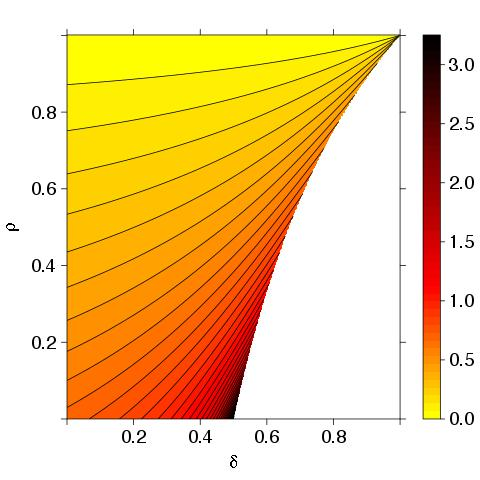
\includegraphics[width=\textwidth]{ExtremeN2}
%%\caption{N = 2}	
%%\label{ExtremeN2}
%%    \end{subfigure}%
%%    \begin{subfigure}[b]{0.499\textwidth}
%%        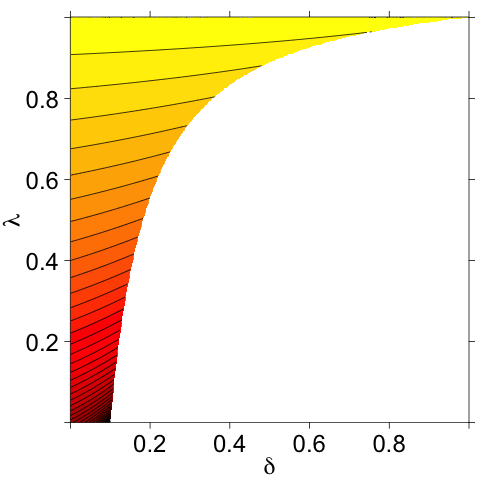
\includegraphics[width=\textwidth]{ExtremeN10}
%%\caption{N = 10}
%%\label{ExtremeN10}
%%    \end{subfigure}
%%    \caption{ The amount of log-extremizing $\log(\alpha)$ under 
%%    different combinations of $N$ (the number of forecasters), 
%%    $\delta$ (the average amount known by one forecaster), and 
%%    $\lambda$ (the average amount shared by any two forecasters).}
%%    \label{Levelplots}
%%\end{figure}
%%\clearpage
% \begin{figure}[h!]
%    \centering
%    \vspace{-1em}
%    \begin{subfigure}[b]{\textwidth}
%\hspace{9em}        \includegraphics{PertLegend}
%\label{legendReal}
%    \end{subfigure}%
%    \vspace{-1em}
%
%    \begin{subfigure}[b]{0.45\textwidth}
%        \includegraphics[width=\textwidth, height = \textwidth]{Real50}
%\caption{$K \geq 50$}	
%\label{real1}
%    \end{subfigure}%
%    \begin{subfigure}[b]{0.45\textwidth}
%        \includegraphics[width=\textwidth, height = \textwidth]{Real100}
%\caption{$K \geq 100$}	
%\label{real2}
%    \end{subfigure}%        
%    \caption{The Brier scores of $p''$ and $\probit(\alpha)$ under super-forecaster data.}
%        \label{RealData}
%\end{figure}
% 
\section{Discussion}
\label{discussion}
This paper introduced a probability model for event forecasts made 
by a group of forecasters.  The model allows for interpretation
of some of the existing work on forecast aggregation and also sheds 
light on empirical approaches such as the {\em ad hoc} practice of extremization.  
The general model is more plausible on the micro-level than any other model has
been to date. Under this model, we provided some general results. For instance,
we showed that the \textit{oracular aggregator} is more likely to give a forecast that is more extreme 
than one of the common benchmark forecasts, namely the probit
opinion pool (Proposition~\ref{positiveProbThm}).  Even though no 
real world aggregator has access to all the information of the 
oracle, the result illuminates why extremization is almost 
certainly called for.  We also performed more detailed analyses under various
specific model specifications such as zero and complete information overlap (Section~\ref{disjoint}), and full
symmetry of the information structure (Section~\ref{compound}).
Even though the zero and complete information overlap models are not realistic, except
under a very narrow set of circumstances, they form logical extremes
that shed light on what drives good aggregation. The symmetric 
model is somewhat more realistic.  Based on its analysis, we 
constructed graphs that illuminated the effect of model parameters 
on the optimal amount of extremization (Figure~\ref{LevelplotsOracle}).
We also considered the {\em revealed aggregator}, which is the
best in-practice aggregation under the partial information model.
We derived a general formula for this aggregator 
(Equation~\ref{GeneralAggregator}), as well as its specific formula 
under the assumption of symmetric information (Equation~\ref{CompoundAggre}).

%It is interesting to relate our discussion to the many empirical 
%studies conducted by the Good Judgment Project %%%(GJP) 
%(\citealt{mellers2014psychological, ungar2012good}).  The GJP is 
%a research study that has recruited thousands of forecasters 
%from professional societies, research centers, and alumni associations. 
%These forecasters are given questions about future international 
%political events, such as who would win an election in Russia or 
%the Congo.  Individuals then estimate the probability of each event, and 
%update their predictions when they feel the probabilities have changed.  
%The forecasters know that their probability estimates are assessed 
%for accuracy using Brier scores, i.e. the squared distance from the  
%probability forecast to $1$ or $0$ depending on whether the event 
%happened or not, respectively (\citealt{Brier}).  This incentivizes 
%the forecasters to report their true beliefs instead of attempting 
%to game the system (\citealt{winkler1968good}).  In addition to receiving 
%\$150 for meeting minimum participation requirements that do not depend 
%on prediction accuracy, the forecasters receive status rewards for 
%their performance via leader-boards displaying Brier scores for the 
%top 20 forecasters.  Every year the top 2\% percent of the forecasters 
%are selected to the elite group of ``super-forecasters''.  The 
%super-forecasters work in groups to make highly accurate predictions 
%on the same events as the rest of the forecasters. 

It is interesting to relate our discussion to the many empirical  studies conducted by the Good Judgment Project (see Section \ref{realData} for a brier introduction of the project).
Generally extremizing has been found to improve the average 
aggregates (\citealt{mellers2014psychological, satopaa, satopaa2014probability}).  The average 
forecast of a team of super-forecasters, however, often 
requires very little or no extremizing.  This can explained by 
the partial information model as follows.  The super-forecasters 
are highly knowledgeable (i.e. they have a high $\delta$) 
and they who work in groups (i.e. they have a high $\rho$ and 
$\lambda$).  In Figure \ref{LevelplotsOracle} 
they are situated around the upper-right corners where almost 
no extremizing is required.  In other words, there is very little
usable information not already used in each forecast.  Their
forecasts are highly convergent and are likely to be already very near
the oracular forecast.  The GJP forecast data also includes 
self-assessments of expertise.  Not surprisingly, the greater
the self=assessed expertise, the less extremizing appears to 
have been required.  This is consistent with our interpretation
that high values of $\delta$ and $\lambda$ lead to a lower
extremization parameter.

%All forecasters were also asked to self-assess their level of expertise (on a $1$-to-$5$ scale with $1$ = Not At All Expert and $5$ = Extremely Expert) on the events for which they provided forecasts. Given that expertise is largely defined by the forecaster's personal knowledge, the value of $\delta$ can be considered positively associated with the self-assessed expertise. Marginally, this implies a positive relationship between the level of expertise and amount of extremizing. \citet{satopaa}, however, suggest that the amount of extremizing is negatively associated with self-assessed expertise, i.e. lower expertise requires more extremizing. This can be explained by two observations. First, the average number of forecasters $N$ per expertise group across the $69$ international events considered in \citet{satopaa} were around $68.3$, $84.9$, $61.6$, $17.5$, and $3.4$ (from the lowest to the highest level of expertise). Second, the low experts had a chance of being highly diverse while the high experts were likely to experience considerable information overlap. These observations suggest that the large low-expertise groups required more extremizing because they held more information in total than the relatively much smaller high-expertise groups.

The partial information framework offers many future research directions. 
One involves estimation of parameters.  It seems likely that use of
this model together with good procedures for estimating the information
overlap among two or more forecasters can lead to many improvements in probability aggregations. Given a stream of forecasts of reasonable length, it is possible to estimate $|B_i|$ and $|B_i \cap B_j|$ with a maximum likelihood procedure akin to details described in Appendix. In principle, the size of $B_i$ can be estimated from 
the distribution of the forecasts $p_{ij}$ and the size of 
$B_i \cap B_j$ from correslations between the $i$th and $j$th 
forecast streams.  Estimation of higher order intersections seems
more dubious.  Computations with $N=3$ show that, at least in some
cases, higher order intersections are not relevant to the
revealed aggregator.  Theoretical results on the significance or 
insignificance of higher order intersections in the information 
overlap structure would be desirable.

Another promising avenue is the Bayesian approach.  Two forecasters
whose forecasts are very similar or perhaps identical are more
likely to have very similar information sets.  In a Bayesian model,
one would expect more extremization from the probit opinion pool
when the set of forecasts is varied than when it is relatively
homogeneous.  We have work in progress analyzing a Bayesian model, but there are many, many reasonable priors 
on information structures.  This avenue should certainly be 
pursued and the results tested against other high performing 
aggregators.


\section*{Acknowledgments} 
This research was supported by a research contract to the University
of Pennsylvania and the University of California from the Intelligence Advanced Research Projects Activity
(IARPA) via the Department of Interior National Business Center
contract number D11PC20061. The U.S. Government is authorized to reproduce and
distribute reprints for Government purposes notwithstanding any
copyright annotation thereon. Disclaimer: The views and conclusions
expressed herein are those of the authors and should not be
interpreted as necessarily representing the official policies or
endorsements, either expressed or implied, of IARPA, DoI/NBC, or the
U.S. Government. 

We deeply appreciate the project management
skills and work of Terry Murray and David Wayrynen, which went far
beyond the call-of-duty on this project. 

\appendix 
\section*{Appendix: Technical Details}
\label{appendix}

\renewcommand{\thesubsection}{\Alph{subsection}}

\subsection{Proofs}
%\textit{Proof of Theorem \ref{positiveThmVote}.} Let $\boldsymbol{d} = \frac{1}{N}\left((1-\delta_1)^{-1/2}, (1-\delta_2)^{-1/2}, \dots, (1-\delta_N)^{-1/2}\right)'$. Assume without loss of generality that $\bar{P} > 0$. Then the average probit forecast is extremized if
%\begin{align}
% \bar{P}&\leq  \frac{\sum_{j=1}^N X_{I_j}}{\sqrt{1 - \sum_{j=1}^N \delta_j}} &\Leftrightarrow&& 0 \leq  \left\{  \left(1 - \sum_{j=1}^N \delta_j \right)^{-1/2} \boldsymbol{1}_N - \boldsymbol{d}' \right\} \boldsymbol{X} \label{votingproof}
%\end{align}
% As $N (1-\delta_j)^{1/2} \geq \left(1 - \sum_{j=1}^N \delta_j \right)^{1/2}$ for all $j = 1, \dots, N$, all the elements of $$\left(1 - \sum_{j=1}^N \delta_j \right)^{-1/2} \boldsymbol{1}_N - \boldsymbol{d}' $$ are non-negative. Therefore the right hand side of (\ref{votingproof}) is always non-negative. \qed
% \
% \\
%\noindent
\subsubsection{Proof of Proposition \ref{positiveProbThm}.}
\begin{align*}
x_0 &= \kappa \frac{\sigma_1}{\sigma_2} \\
 &= \frac{ \sum_{i=1}^N \frac{\delta_i}{\sqrt{1-\delta_i}}}{\sqrt{\delta'  \left\{ \sum_{i=1}^N \frac{\delta_i}{1-\delta_i} + 2 \sum_{i,j: i<j} \frac{\rho_{ij}}{\sqrt{(1-\delta_j)(1-\delta_i)}}\right\}}} \sqrt{\frac{\frac{\delta'}{1-\delta'}}{\frac{1}{N^2} \left\{ \sum_{i=1}^N \frac{\delta_i}{1-\delta_i} + 2 \sum_{i,j: i<j} \frac{\rho_{ij}}{\sqrt{(1-\delta_j)(1-\delta_i)}}\right\} }}\\
%&=  \frac{N \sum_{j=1}^N \frac{\delta_j}{\sqrt{1-\delta_j}}}{\sqrt{ \left( \sum_{j=1}^N \frac{\delta_j}{1-\delta_j} + 2 \sum_{i,j: i<j} \frac{\rho_{ij}}{\sqrt{(1-\delta_j)(1-\delta_i)}}\right)}} \sqrt{\frac{\frac{1}{1-\delta'}}{ \left( \sum_{j=1}^N \frac{\delta_j}{1-\delta_j} + 2 \sum_{i,j: i<j} \frac{\rho_{ij}}{\sqrt{(1-\delta_j)(1-\delta_i)}}\right) }}\\
%&=  \frac{N \sum_{j=1}^N \frac{\delta_j}{\sqrt{1-\delta_j}}}{ \sum_{j=1}^N \frac{\delta_j}{1-\delta_j} + 2 \sum_{i,j: i<j} \frac{\rho_{ij}}{\sqrt{(1-\delta_j)(1-\delta_i)}}} \sqrt{\frac{1}{1-\delta'}}\\
&=  \frac{N \sum_{i=1}^N \frac{\delta_i}{\sqrt{(1-\delta_i)(1-\delta')}}}{ \sum_{i=1}^N \frac{\delta_i}{1-\delta_i} + 2 \sum_{i,j: i<j} \frac{\rho_{ij}}{\sqrt{(1-\delta_j)(1-\delta_i)}}}
%&\geq  1
%&=  \frac{\frac{1}{N} \sum_{j=1}^N \frac{\delta_j}{\sqrt{(1-\delta_j)(1-\delta')}}}{\frac{1}{N^2} \left( \sum_{j=1}^N \frac{\delta_j}{1-\delta_j} + 2 \sum_{i,j: i<j} \frac{\rho_{ij}}{\sqrt{(1-\delta_j)(1-\delta_i)}} \right)}\\
\end{align*}
Given that all the remaining terms are positive, the location parameter $x_0$ is also positive. Next compare the $N$ terms with a given subindex $i$ in the numerator with the corresponding terms in the denominator. From $\delta' \geq \delta_i \geq \rho_{ij}$ it follows that 
\begin{align}
\frac{\delta_i}{1-\delta_i} = \frac{\delta_i}{\sqrt{(1-\delta_i)(1-\delta_i)}} &\leq \frac{\delta_i}{\sqrt{(1-\delta_i)(1-\delta')}} \label{ProofIneq1}\\
 \frac{\rho_{ij}}{\sqrt{(1-\delta_j)(1-\delta_i)}} &\leq \frac{\delta_i}{\sqrt{(1-\delta_i)(1-\delta')}} \label{ProofIneq2}
\end{align}
Therefore 
\begin{align*}
N \sum_{i=1}^N \frac{\delta_i}{\sqrt{(1-\delta_i)(1-\delta')}} \geq \sum_{i=1}^N \frac{\delta_i}{1-\delta_i} + 2 \sum_{i,j: i<j} \frac{\rho_{ij}}{\sqrt{(1-\delta_j)(1-\delta_i)}},
\end{align*}
which gives that $x_0 \geq 1$. Given that the Cauchy distribution is symmetric around $x_0$, it must be the case that $\P(\alpha \geq 1 | \Sigma_{22}, \delta') \geq 0.5$. Based on (\ref{ProofIneq1}) and (\ref{ProofIneq2}), the location $x_0 = 1$ only when all the forecasters know the same information, i.e. when $\delta_i = \delta'$ for all $i = 1, \dots, N$. Under this particular setting, the amount of extremizing $\alpha$ is non-random and always equal to $1.0$. Therefore $\P(\alpha \geq 1 | \Sigma_{22}, \delta') = 1.0$.  Any deviation from this particular information structure makes $\alpha$ stochastic, $x_0 > 1$, and hence $\P(\alpha \geq 1 | \Sigma_{22}, \delta') > 0.5$. If the forecasters' information sets partition the full information, the sum of their probits is always on the correct side of $0.0$. At the same time the oracle deterministically outputs the correct outcome. Consequently, $\alpha = +\infty$ and $\P(\alpha \geq 1 | \Sigma_{22}, \delta') = 1$. Thus $\P(\alpha > 1 | \Sigma_{22}, \delta') \in (0.5, 1.0]$ when $\delta_i \neq \delta'$ for some $i = 1, \dots, N$. \qed
%\noindent
%\textit{Proof of Proposition \ref{positiveThmVote}.} Let $\boldsymbol{d} = \frac{1}{N}\left((1-\delta_1)^{-1/2}, (1-\delta_2)^{-1/2}, \dots, (1-\delta_N)^{-1/2}\right)'$. Assume without loss of generality that $\bar{P} > 0$. Then the average probit forecast is extremized if
%\begin{align}
% \bar{P}&\leq  \frac{\sum_{j=1}^N X_{I_j}}{\sqrt{1 - \sum_{j=1}^N \delta_j}} &\Leftrightarrow&& 0 \leq  \left\{  \left(1 - \sum_{j=1}^N \delta_j \right)^{-1/2} \boldsymbol{1}_N - \boldsymbol{d}' \right\} \boldsymbol{X} \label{votingproof}
%\end{align}
% As $N (1-\delta_j)^{1/2} \geq \left(1 - \sum_{j=1}^N \delta_j \right)^{1/2}$ for all $j = 1, \dots, N$, all the elements of $$\left(1 - \sum_{j=1}^N \delta_j \right)^{-1/2} \boldsymbol{1}_N - \boldsymbol{d}' $$ are non-negative. Therefore the right hand side of (\ref{votingproof}) is always non-negative. \qed
%\\
%\\
\subsubsection{Proof of Proposition \ref{positiveThm}.}

\begin{enumerate}
\item[(i)] This follows from direct computation,
\begin{align}
\alpha &= \left( \frac{\frac{1}{(N-1)\lambda +1} 
  \sum_{i=1}^N X_{I_i} }{\sqrt{1- \frac{N\delta}{(N-1)\lambda +1} }} \right) \Big/ \left( \frac{1}{N} \sum_{i=1}^N \frac{X_{I_i}}{\sqrt{1-\delta}} \right) \nonumber \\
&=    \frac{\frac{N\sqrt{1-\delta}}{(N-1)\lambda +1} 
   }{\sqrt{1- \frac{N\delta}{(N-1)\lambda +1} }}, \label{CompoundAlpha}
\end{align}
which simplifies to the given expression after substituting in $\gamma$. This quantity does not depend on any $X_{I_i}$ and is therefore non-random.

\item[(ii)] For a given $\delta$, the amount of extremizing $\alpha$ is minimized when $(N-1)\lambda +1$ is maximized. This happens as $\lambda \uparrow 1$. Plugging this into (\ref{CompoundAlpha}) gives
\begin{align*}
\alpha &= \frac{\frac{N\sqrt{1-\delta}}{(N-1)\lambda +1}}{\sqrt{1- \frac{N\delta}{(N-1)\lambda +1} }}  \downarrow \frac{\sqrt{1-\delta}}{\sqrt{1-\delta }} = 1
\end{align*}
\item[(iii)] Assume without loss of generality that $\bar{P} > 0$. If $\max\{p_1, p_2, \dots, p_N \} < 1$, then  setting $\delta = 1/N$ and $\lambda = 0$ gives an aggregate probability $p'' = 1$ that is outside the convex hull of the individual probabilities.
\qed
\end{enumerate}

\subsection{Parameter Estimation under Symmetric Information}
%The information among $N=2$ forecasters is completely characterized by $\delta_1$, $\delta_2$, and $\rho_{12}$. The values of these parameters can be estimated via the maximum likelihood method.  To make this more explicit, observe that the Jacobian for the map $\boldsymbol{P} \to \Phi\left(\boldsymbol{P}\right) = (\Phi(P_1), \Phi(P_2))'$ is
%\begin{eqnarray*}
%J(\boldsymbol{P}) &=& (2\pi)^{-1} \exp \left( - \frac{\boldsymbol{P}' \boldsymbol{P}}{2}   \right) 
%\end{eqnarray*}
%%
%%$\boldsymbol{P} \sim \mathcal{N}_N\left(\boldsymbol{0}, \Sigma_{22} (1-\delta)^{-1}\right)$ and that
%Let $t = \Phi^{-1}(1-\tilde{p})$. Then, if $h(\boldsymbol{P})$ denotes the multivariate Gaussian density of $\boldsymbol{P} \sim \mathcal{N}_2\left(-t/\sqrt{1-\boldsymbol{\delta}}, \Sigma_{P}\right)$,
%%by the Inverse Function Theorem 
%the density for  $\boldsymbol{p} = (p_1, p_2)'$ becomes
%\begin{eqnarray*}
%&& f\left(\boldsymbol{p} | \delta_1, \delta_2, \rho \right) \\
% &=& h(\boldsymbol{P}) J(\boldsymbol{P})^{-1} \\
%% \bigg|_{\boldsymbol{P} = \Phi^{-1}(\boldsymbol{p})}\\
%%&=& \frac{(1-\delta)^{N/2}}{\sqrt{ |\Sigma_{22}|}} \exp\left( -\frac{1}{2} \boldsymbol{P}' (1-\delta)\Sigma_{22}^{-1} \boldsymbol{P} + \frac{\boldsymbol{P}' \boldsymbol{P}}{2}   \right)\\
%&=& \frac{1}{\sqrt{ \left|\Sigma_{P}\right|}} \exp\left[ -\frac{1}{2} \left[ \left( \boldsymbol{P} + t/\sqrt{1-\boldsymbol{\delta}}\right)' \Sigma_{P}^{-1}  \left(\boldsymbol{P} + t/\sqrt{1-\boldsymbol{\delta}}\right) -  \boldsymbol{P}'\boldsymbol{P}\right] \right],
%\end{eqnarray*}
%where $\Phi^{-1}(\boldsymbol{p}) = \boldsymbol{P}$. Assume that the forecasters participated in $K$ problems. If the forecasts given for the $k$th problem are denoted with $\boldsymbol{p}_k$, then the maximum likelihood estimates of $\delta_1$, $\delta_2$, and $\rho$ are obtained from
%\begin{align*}
%\left(\hat{\delta}_1, \hat{\delta}_2, \hat{\rho}\right) =& \argmax_{\delta_1, \delta_2, \rho} \sum_{k=1}^K \log  f\left(\boldsymbol{p}_k| \delta_1, \delta_2, \rho \right),\\
%& \text{s.t. } \nonumber \delta_1, \delta_2 \in [0,1] \text{ and } \rho \in \left[  \max \left\{\delta_1+\delta_2 - 1,  0\right\}, \min \left\{\delta_1, \delta_2 \right\} \right]
%\end{align*}
%This works well as long as the forecasters participate in the same set of problems. The forecasters, however, were allowed to choose their problems and therefore generally do not participate in the same set of problems. Disregarding any problems with partial participation would lead to a loss of information. Therefore it is necessary to handle the missing values in some manner. The first step is to assume that the forecasts are missing at random. The likelihood for a unpaired forecast, say $p_j$, then is the marginal likelihood of $p_j$
%\begin{align*}
%%&& f\left(p_1 | \delta_1, \delta_2, \rho \right) \\
% m(p_j | \delta_j) &= \sqrt{\frac{1-\delta_j}{\delta_j}} \exp  \left\{ \frac{\delta_jP_j^2- (1-\delta_j)(P_j + t/\sqrt{1-\delta_j})^2 }{2\delta_j}  \right\},
%%&=& \frac{1}{\sqrt{ \left|\Sigma_{P}\right|}}  \int_0^1  \exp\left[ -\frac{1}{2} \Phi^{-1}(\boldsymbol{p})'\Lambda \Phi^{-1}(\boldsymbol{p})  \right] dp_2\\
%%%&=& \frac{1}{\sqrt{ \left|\Sigma_{P}\right|}}   \int_0^1  \exp\left[ -\frac{1}{2} \left( \Phi^{-1}(p_1)^2\Lambda_{11} + \Phi^{-1}(p_1)\Phi^{-1}(p_2)(\Lambda_{12}+\Lambda_{21}) +  \Phi^{-1}(p_2)^2\Lambda_{22} \right) \right] dp_2\\
%%%&=& \frac{1}{\sqrt{ \left|\Sigma_{P}\right|}}    \exp\left[ -\frac{1}{2}  P_1^2\Lambda_{11} \right]  \int_0^1  \exp\left[ -\frac{1}{2} \left( P_1\Phi^{-1}(p_2)(\Lambda_{12}+\Lambda_{21}) +  \Phi^{-1}(p_2)^2\Lambda_{22} \right) \right] dp_2\\
%%&=& \frac{1}{\sqrt{ \left|\Sigma_{P}\right|}}    \exp\left[ -\frac{1}{2}  P_1^2\Lambda_{11} \right]  \int_{-\infty}^\infty  \exp\left[ -\frac{1}{2} \left( P_1 P_2(\Lambda_{12}+\Lambda_{21}) +  P_2^2\Lambda_{22} \right) \right] \phi(P_2) dP_2\\
%%%&=& \frac{1}{\sqrt{ 2\pi \left|\Sigma_{P}\right|}}    \exp\left[ -\frac{1}{2}  P_1^2\Lambda_{11} \right]  \int  \exp\left[ -\frac{1}{2} \left( P_2 P_1 (\Lambda_{12}+\Lambda_{21}) +  P_2^2\Lambda_{22} \right) - \frac{1}{2} P_2^2\right]  dP_2\\
%%%&=& \frac{1}{\sqrt{ 2\pi \left|\Sigma_{P}\right|}}    \exp\left[ -\frac{1}{2}  P_1^2\Lambda_{11} \right]  \int  \exp\left[ -\frac{1}{2} \left( P_2 P_1 (\Lambda_{12}+\Lambda_{21}) +  P_2^2(\Lambda_{22}+1) \right) \right]  dP_2\\
%%%&=& \frac{1}{\sqrt{ 2\pi \left|\Sigma_{P}\right|}}    \exp\left[ -\frac{1}{2}  P_1^2\Lambda_{11} \right]  \frac{2.50663 \exp\left(\frac{0.5P_1^2 \Lambda_{12}^2}{\Lambda_{22}+1}\right)}{\sqrt{\Lambda_{22}+1}}\\
%%&=& \frac{2.50663}{\sqrt{ 2\pi \left|\Sigma_{P}\right|(\Lambda_{22}+1)}}    \exp\left[ -\frac{1}{2}  P_1^2\left( \Lambda_{11} - \frac{\Lambda_{12}^2}{\Lambda_{22}+1}\right) \right] \\
%%\end{eqnarray*}
%%Assume that $ \Sigma_{P}^{-1} - I_2$ is invertible and let $\Lambda = ( \Sigma_{P}^{-1} - I_2)^{-1}$. Then,
%%\begin{eqnarray*}
%% f\left(p_1 | \delta_1, \delta_2, \rho \right) &=&  2\pi \sqrt{ \frac{|\Lambda|}{|\Sigma_{P}|}} \int_{\mathbb{R}} \frac{1}{2\pi \sqrt{|\Lambda|}} \exp\left( -\frac{1}{2} \boldsymbol{P}' \Lambda^{-1} \boldsymbol{P}  \right) dP_2\\
%% &=&  2\pi  \sqrt{ \frac{|\Lambda|}{|\Sigma_{P}|}} \phi(p_1 | 0, \Lambda_{11}),
%\end{align*}
%where $P_j = \Phi^{-1}(p_j)$. 
%%where $\Lambda_{11}$ is the $(1,1)$th element of $\Lambda$ and $\phi(\cdot | \mu, \sigma^2)$ represents the probability density function of a normal distribution with mean $\mu$ and variance $\sigma^2$.
%%By symmetry, the likelihood $f\left(p_2 | \delta_1, \delta_2, \rho \right)$ follows similarly.  
%Let $\mathcal{K}_{12}$ denote the set of problems in which both forecasters participated. Similarly, let $\mathcal{K}_1$ and $\mathcal{K}_2$ denote the sets of problems in which only Forecaster $1$ and $2$ participated, respectively. The final optimization task then becomes
%\begin{align*}
%\left(\hat{\delta}_1, \hat{\delta}_2, \hat{\rho}\right) =& \argmax_{\delta_1, \delta_2, \rho} \left\{ \sum_{k \in \mathcal{K}_{12}} \log  f\left(\boldsymbol{p}_k| \delta_1, \delta_2, \rho \right) +  \sum_{j = 1}^2 \sum_{k \in \mathcal{K}_{j}} \log  m\left(p_j| \delta_j \right)  \right\},\\
%& \text{s.t. } \nonumber \delta_1, \delta_2 \in [0,1] \text{ and } \rho \in \left[  \max \left\{\delta_1+\delta_2 - 1,  0\right\}, \min \left\{\delta_1, \delta_2 \right\} \right]
%\end{align*}
%The feasible set of parameter values is described by the intersection of four half spaces. Therefore this optimization problem can be efficiently solved via generic techniques such as the barrier method (see, e.g., \cite{boyd2009convex} for more information). 
%%Given that this optimization problem cannot be solved analytically, numerical methods must be used. The feasible set of parameter values is a convex set defined by the intersection of four half-spaces. Therefore the constraints are equivalent to a set of linear inequalities
%%\begin{align*}
%%-\rho &\leq 0\\
%%\delta_1+\delta_2-\rho-1 &\leq 0\\
%%\rho - \delta_1 &\leq 0\\
%%\rho - \delta_2 &\leq 0
%%\end{align*}
%%and an adaptive barrier method can be used to solve the maximization problem. 
%%\subsection*{A.3 Estimation of $\delta$ and $\lambda$}


The values of $\delta$ and $\lambda$ can be estimated via the maximum likelihood method. To make this more explicit, observe that the Jacobian for the map $\boldsymbol{P} \to \Phi\left(\boldsymbol{P}\right) = (\Phi(P_1), \Phi(P_2), \dots, \Phi(P_N))'$ is
\begin{eqnarray*}
J(\boldsymbol{P}) &=& (2\pi)^{-N/2} \exp \left( - \frac{\boldsymbol{P}' \boldsymbol{P}}{2}   \right) 
\end{eqnarray*}
%
%$\boldsymbol{P} \sim \mathcal{N}_N\left(\boldsymbol{0}, \Sigma_{22} (1-\delta)^{-1}\right)$ and that
Let $J_{N \times N}$ represent a $N\times N$ matrix of ones. If $h(\boldsymbol{P})$ denotes the multivariate Gaussian density of $\boldsymbol{P} \sim \mathcal{N}_N\left(\boldsymbol{0}, \Sigma_{22} (1-\delta)^{-1}\right)$,
%by the Inverse Function Theorem 
the density for  $\boldsymbol{p} = (p_1, p_2, \dots, p_N)'$ becomes
\begin{eqnarray*}
 f\left(\boldsymbol{p} | \delta, \lambda \right) &=& h(\boldsymbol{P}) J(\boldsymbol{P})^{-1} \bigg|_{\boldsymbol{P} = \Phi^{-1}(\boldsymbol{p})}\\
%&=& \frac{(1-\delta)^{N/2}}{\sqrt{ |\Sigma_{22}|}} \exp\left( -\frac{1}{2} \boldsymbol{P}' (1-\delta)\Sigma_{22}^{-1} \boldsymbol{P} + \frac{\boldsymbol{P}' \boldsymbol{P}}{2}   \right)\\
&=& \frac{(1-\delta)^{N/2}}{\sqrt{ \left|\Sigma_{22}\right|}} \exp\left[ -\frac{1}{2} \Phi^{-1}(\boldsymbol{p})' \left\{ (1-\delta) \Sigma_{22}^{-1} - I_N \right\} \Phi^{-1}(\boldsymbol{p})  \right],
\end{eqnarray*}
%where $\Phi^{-1}(\boldsymbol{p}) =  (\Phi^{-1}(p_1), \Phi^{-1}(p_2), \dots, \Phi^{-1}(p_N))$. 
%Given that $\Sigma_{22}$ can be written in the form  $\Sigma_{22} = I_N (\delta-\lambda\delta) + J_{N \times N} \lambda\delta$
where
%The determinant and inverse of $\Sigma_{22}$ are
\begin{align}
\left| \Sigma_{22}\right| &= (\delta(1- \lambda))^N \left(1+\frac{N \lambda}{1 - \lambda} \right) \nonumber\\
\Sigma_{22}^{-1} &= I_N \left(\frac{1}{\delta-\lambda\delta} \right) - J_{N \times N} \frac{\lambda}{(1-\lambda)\delta\{1+(N-1) \lambda\}} \label{inverse}
\end{align}
See \citet{rao2009linear} and the supplementary material of \citet{dobbin2005sample} for the derivations of the determinant and inverse of $\Sigma_{22}$, respectively. The maximum likelihood estimates of $\delta$ and $\lambda$ are then obtained from
\begin{align*}
\left(\hat{\delta}, \hat{\lambda}\right) =& \argmax_{\lambda, \delta} \log  f\left(\boldsymbol{p}| \delta, \lambda \right),\\
& \text{s.t. } \nonumber \delta \in [0,1] \text{ and } \lambda \in \left[  \max \left\{ \frac{N-\delta^{-1}}{N-1}, 0\right\}, 1 \right)
\end{align*}
%\textcolor{red}{check if this is a convex program}
Given that this cannot be solved analytically, numerical methods such as a simple grid-search or the barrier method must be used to find $\hat{\delta}$ and $\hat{\lambda}$. 

% 
%\subsection*{A.3 Rotating the Calibration Curve}
%The calibrated probabilities follow
%\begin{align*}
%p_{jk} |Y_k &\stackrel{iid}{\sim} \begin{cases}
%2p_{jk}& \text{ if } Y_k = 1\\
%2(1-p_{jk})& \text{ if } Y_k = 0,
%\end{cases}
%\end{align*}
%To introduce under- and overconfidence, this density is rotated counter- or clockwise, respectively, by some amount $\theta \in \left[-(\frac{\pi}{2} - \tan^{-1}(2), \tan^{-1}(2)\right]$. 
%The rotated density for $p_{jk} |Y_k, \theta$ is
%\begin{align}
%f(p_{jk} |Y_k, \theta) &=
%% 1+(-1)^{Y_k}R(\theta)(0.5-p_{jk})
%\begin{cases}
%c(\theta)\left[1+R(\theta)(p_{jk}-0.5) \right]& \text{ if } Y_k = 1\\
%c(\theta)\left[1+R(\theta)(0.5-p_{jk})\right]& \text{ if } Y_k = 0,
%\end{cases}
%\label{rotatedDens}
%\end{align}
%where 
%\begin{align*}
%R(\theta) &= \frac{2\cos(\theta)-\sin(\theta)}{\cos(\theta) + 2\sin(\theta)},
%\end{align*}
%and $c(\theta)$ is a normalizing constant that depends on $\theta$.  The domain of $p_{jk}$  also depends on $\theta$. In particular, if $\theta \geq 0$, then $c(\theta) = 1$ and $p_{ij} \in [0,1]$. If, on the other hand, $\theta < 0$, then $c(\theta) = R(\theta)/2$ and $p_{ij} \in [l,u]$, where $l = 0.5-R(\theta)^{-1}$ and $u = 0.5+R(\theta)^{-1}$. Given that $\P(Y_{jk} = 1) = 0.5$, marginalizing out $Y_{jk}$ gives
%\begin{align*}
%m(p_{jk} | \theta) &= 0.5f(p_{jk} |Y_k=0, \theta) + 0.5f(p_{jk} |Y_k=1, \theta)\\
%&= c(\theta)
%\end{align*}
%Therefore $p_{jk} | \theta$ is uniform over its domain. It is possible to sample from (\ref{rotatedDens}) using the inverse transform sampling method. More specifically, to make a single draw, begin by generating a uniform random variable $u \sim \mathcal{U}[0,1]$. This can be turned into a draw $p$ from (\ref{rotatedDens}) via the following solution to a second degree polynomial 
%\begin{align*}
%p &= \frac{-B+\sqrt{B^2-4AC}}{2A},
%\end{align*}
%where 
%\begin{align*}
%A &= \begin{cases}
%(-1)^{1-Y_{jk}} R(\theta)/2 & \text{ if } \theta \geq 0\\
%(-1)^{1-Y_{jk}} R(\theta)^2/4& \text{ if } \theta < 0
%\end{cases}\\
%B &= \begin{cases}
%1+(-1)^{Y_{jk}} R(\theta)/2 & \text{ if } \theta \geq 0\\
%R(\theta)/2\left(1- (-1)^{1-Y_{jk}} R(\theta)/2\right)& \text{ if } \theta < 0
%\end{cases}\\
%C &= \begin{cases}
%-u & \text{ if } \theta \geq 0\\
%-R(\theta)l +R(\theta)^2/4(-1)^{1-Y_{jk}}l(1-l) - u & \text{ if } \theta < 0
%\end{cases}
%\end{align*}


%\bibliographystyle{Chicago}
%\bibliographystyle{plainnat}
\bibliographystyle{chicago}
\bibliography{biblio}		% expects file ''myrefs.bib''



\end{document}
